\begin{figure*}
\begin{minipage}[t]{0.33\linewidth}%
\begin{framed}
\setcounter{subfigure}{0}
\begin{minipage}[t]{0.49\textwidth}%
\centering
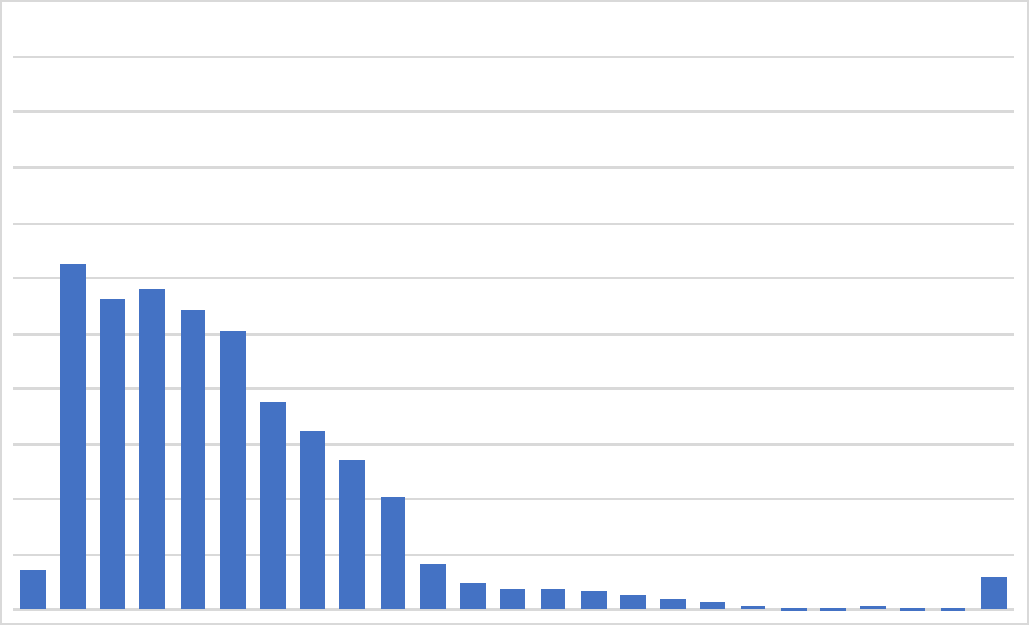
\includegraphics[width=0.95\textwidth]{results/sw4/Eul1_AvgL2.pdf}%
\vspace{-3mm}
\captionof{subfigure}{\footnotesize{Eul 250 Avg$_{L2}$}}
\end{minipage}%
\hfill
\begin{minipage}[t]{0.49\textwidth}%
\centering
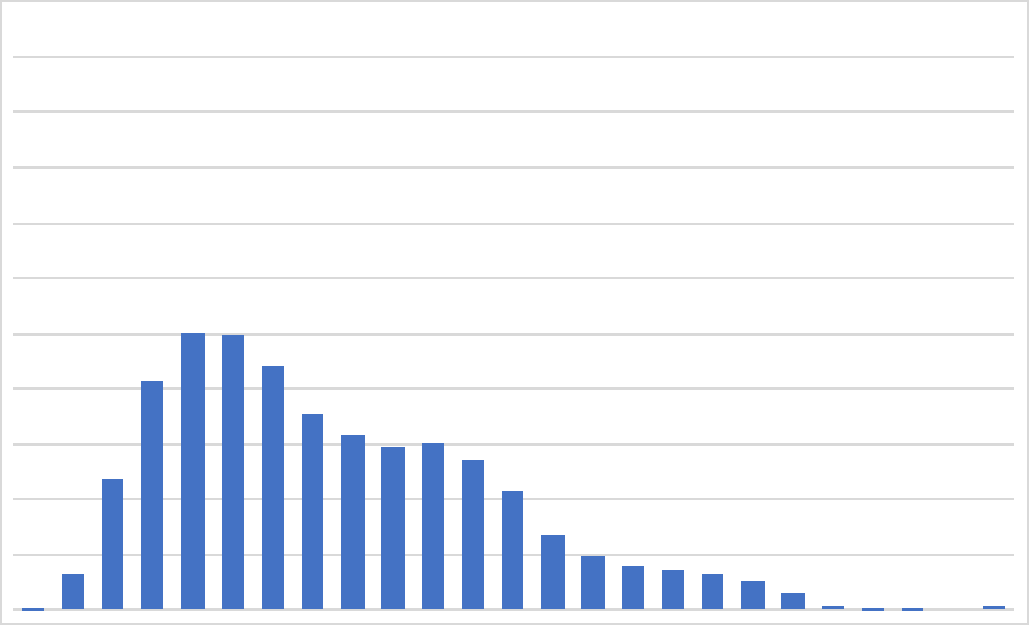
\includegraphics[width=0.95\linewidth]{results/sw4/Eul2_AvgL2.pdf}
\vspace{-3mm}
\captionof{subfigure}{\footnotesize{Eul 500 Avg$_{L2}$}} 
\end{minipage}
\begin{minipage}[t]{0.49\textwidth}%
\centering
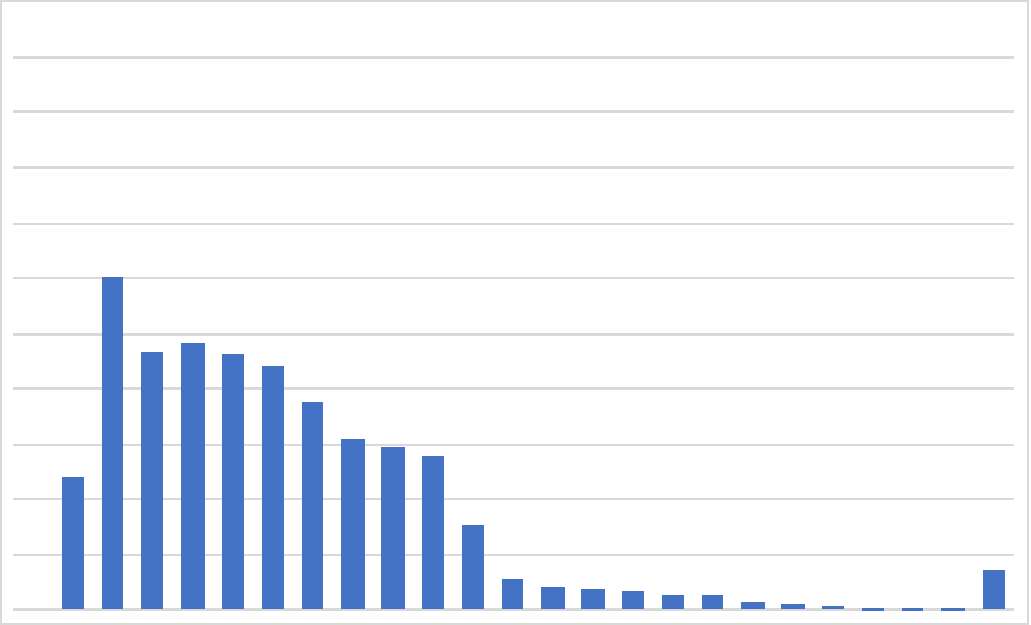
\includegraphics[width=0.95\textwidth]{results/sw4/Eul1_Max.pdf}%
\vspace{-3mm}
\captionof{subfigure}{\footnotesize{Eul 250 Max$_{L2}$}}
\end{minipage}%
\hfill
\begin{minipage}[t]{0.49\textwidth}%
\centering
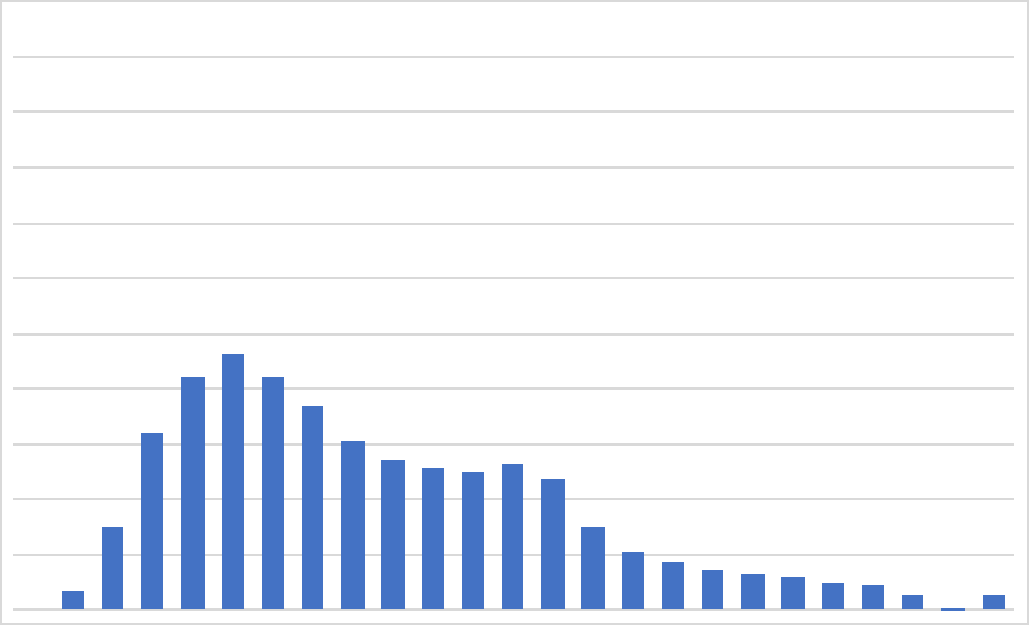
\includegraphics[width=0.95\linewidth]{results/sw4/Eul2_Max.pdf}
\vspace{-3mm}
\captionof{subfigure}{\footnotesize{Eul 500 Max$_{L2}$}} 
\end{minipage}
\begin{minipage}[t]{0.49\textwidth}%
\centering
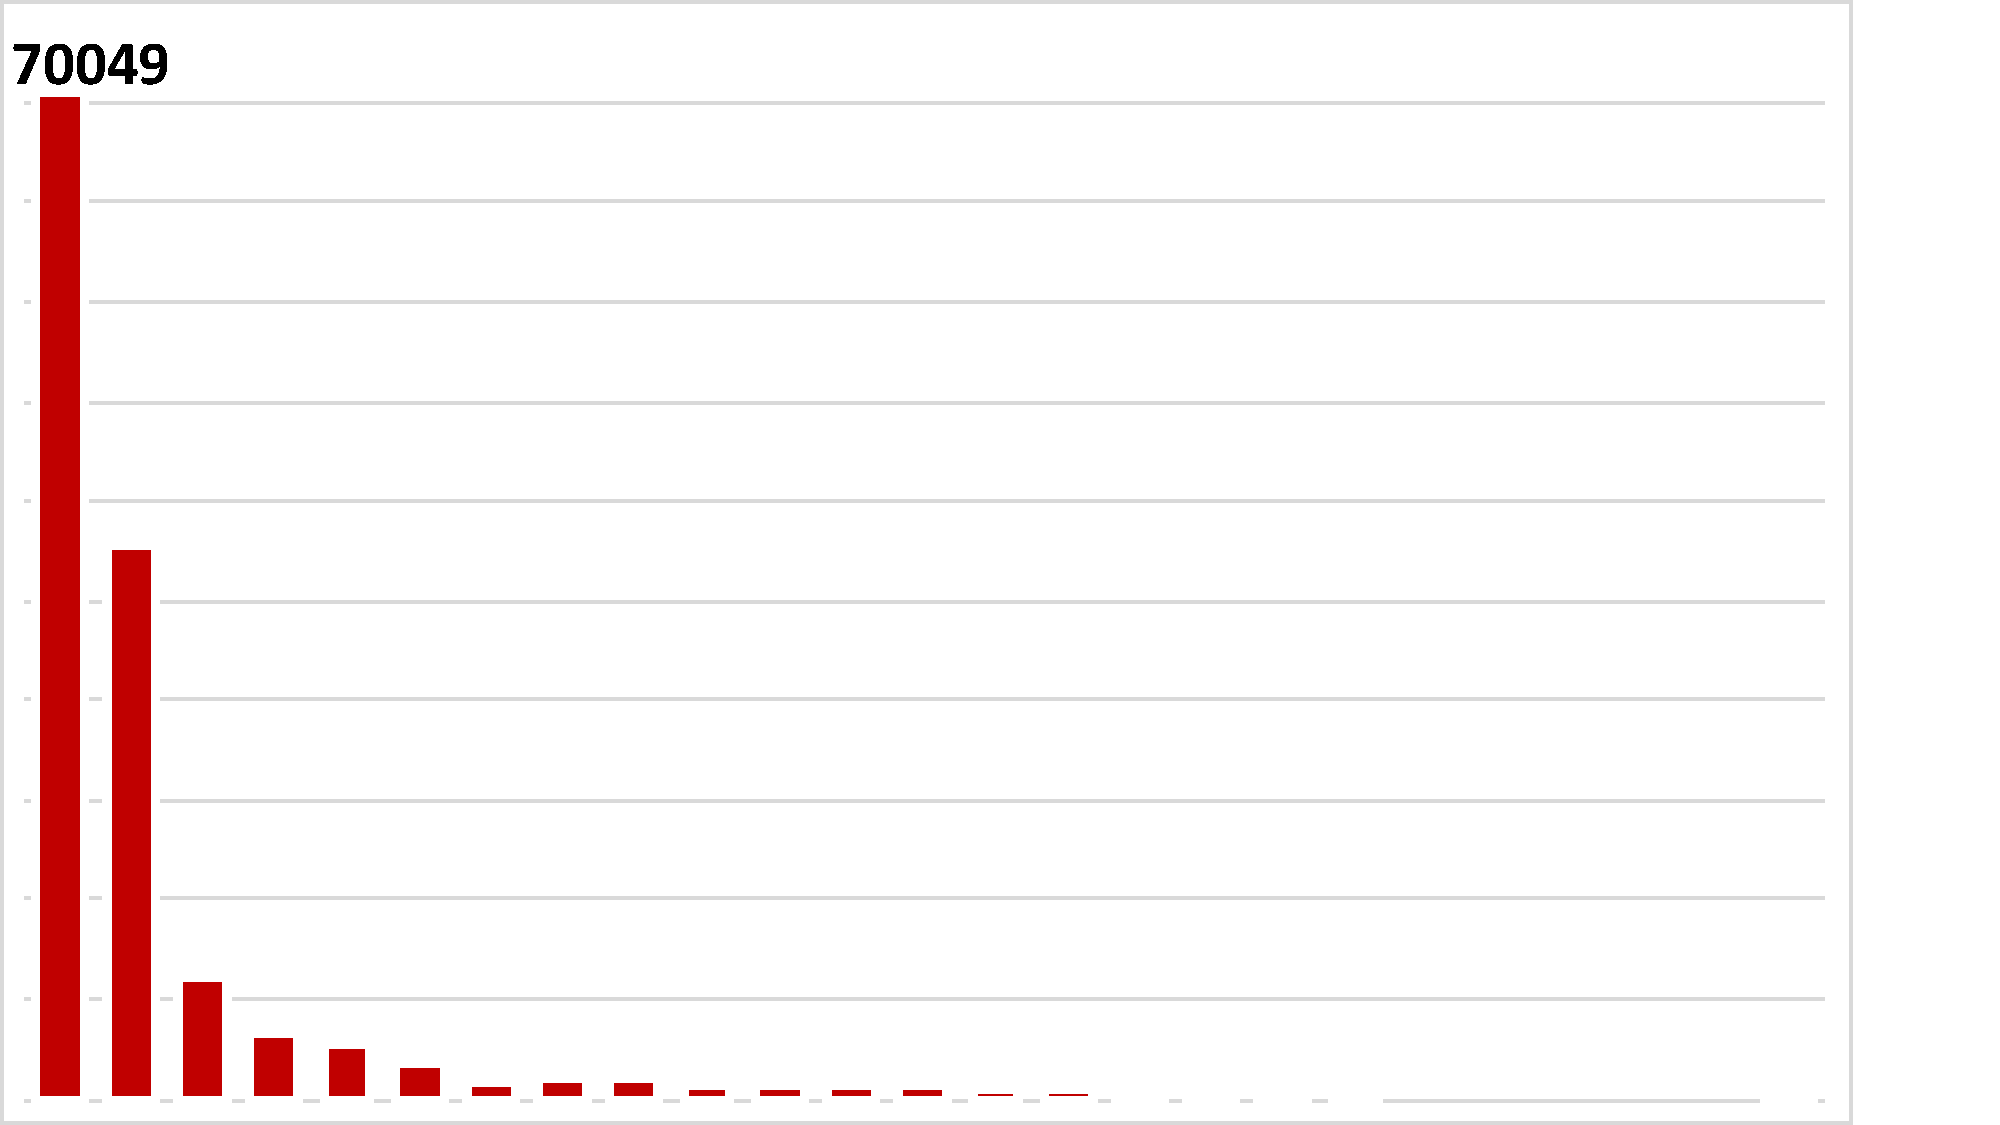
\includegraphics[width=0.95\linewidth, trim={0cm 0cm 2.5cm 0cm}, clip]{results/sw4/Lag3_AvgL2.pdf}
\vspace{-3mm}
\captionof{subfigure}{\footnotesize{Lag 250 1:27 Avg$_{L2}$}}
\end{minipage}%
\hfill
\begin{minipage}[t]{0.49\textwidth}%
\centering
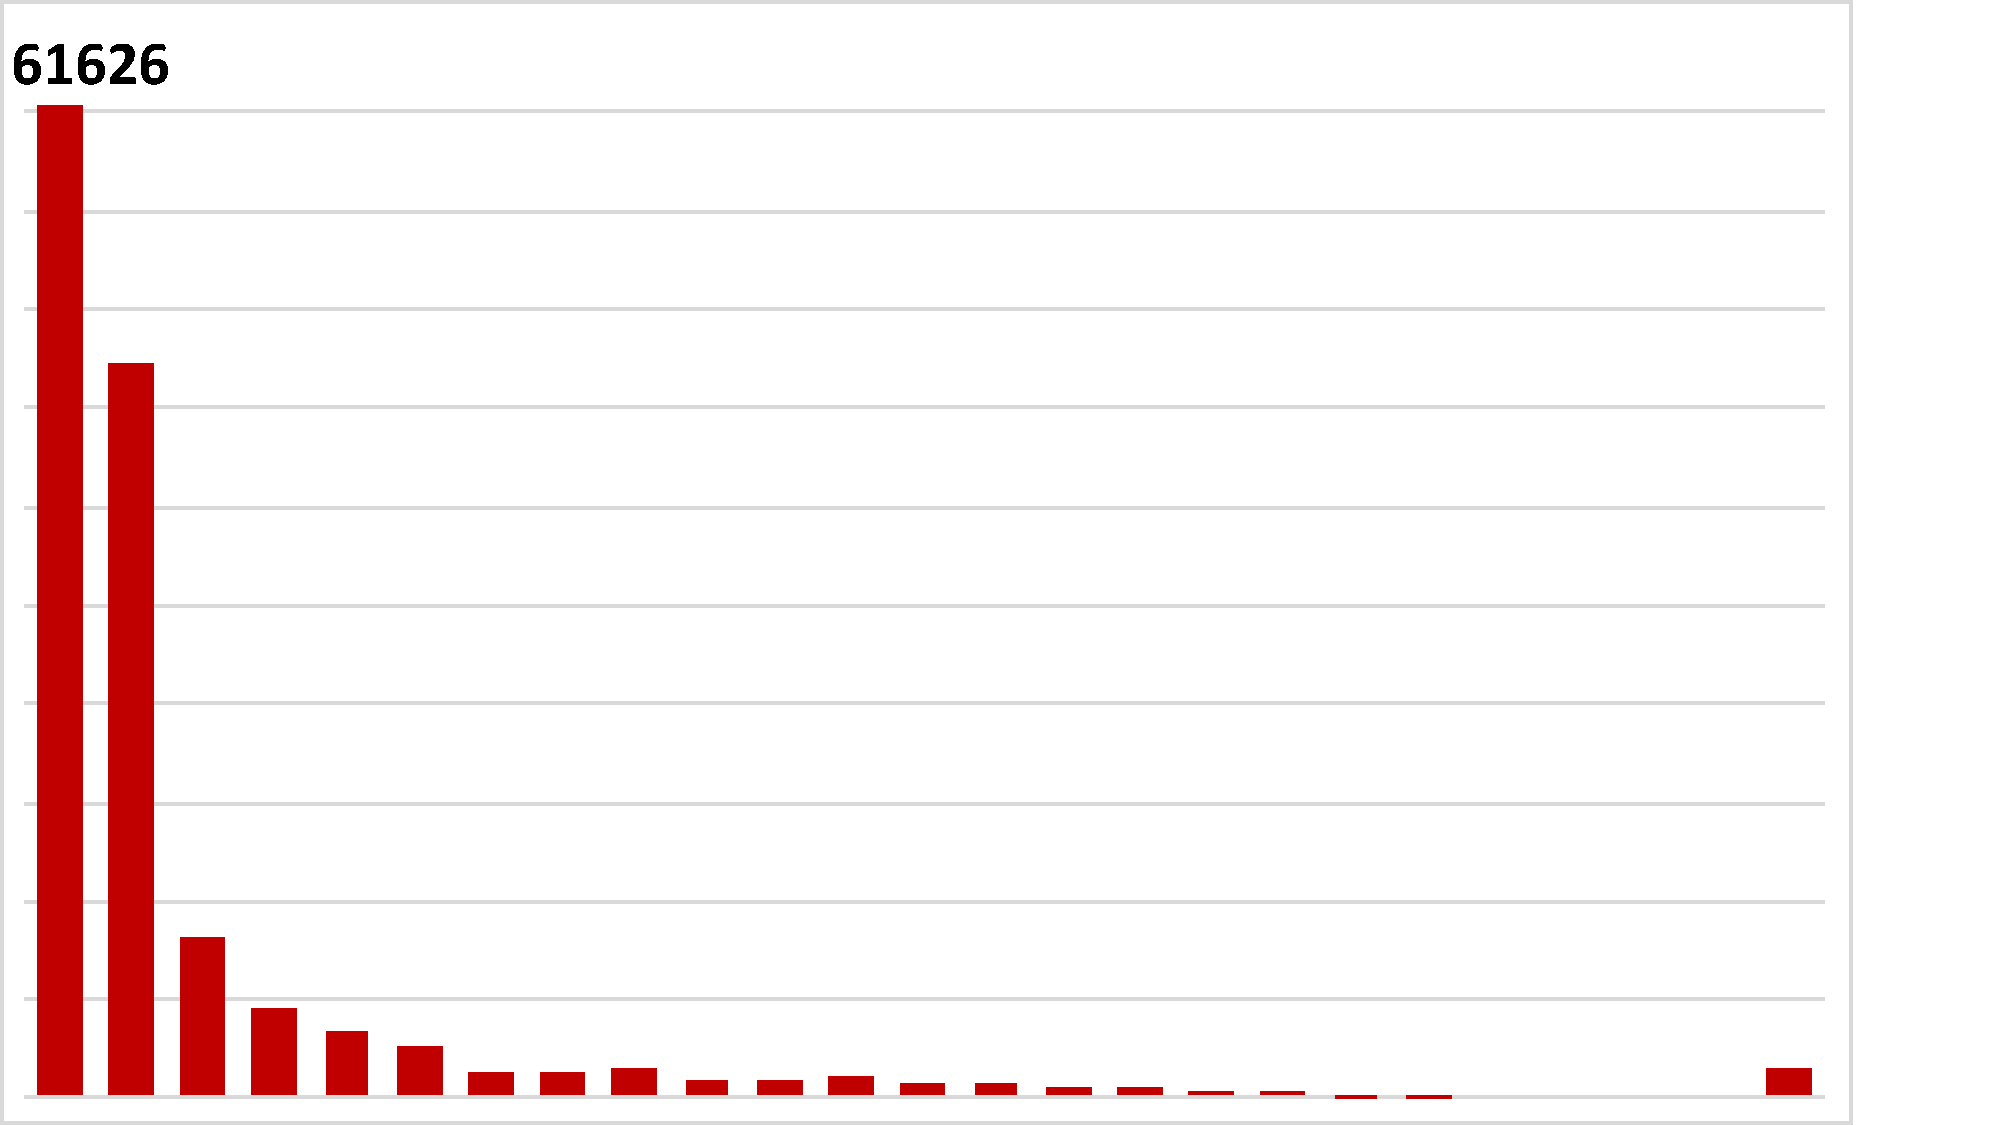
\includegraphics[width=0.95\linewidth, trim={0cm 0cm 2.5cm 0cm}, clip]{results/sw4/Lag4_AvgL2.pdf}
\vspace{-3mm}
\captionof{subfigure}{\footnotesize{Lag 250 1:64 Avg$_{L2}$}} 
\end{minipage}
\begin{minipage}[t]{0.49\textwidth}%
\centering
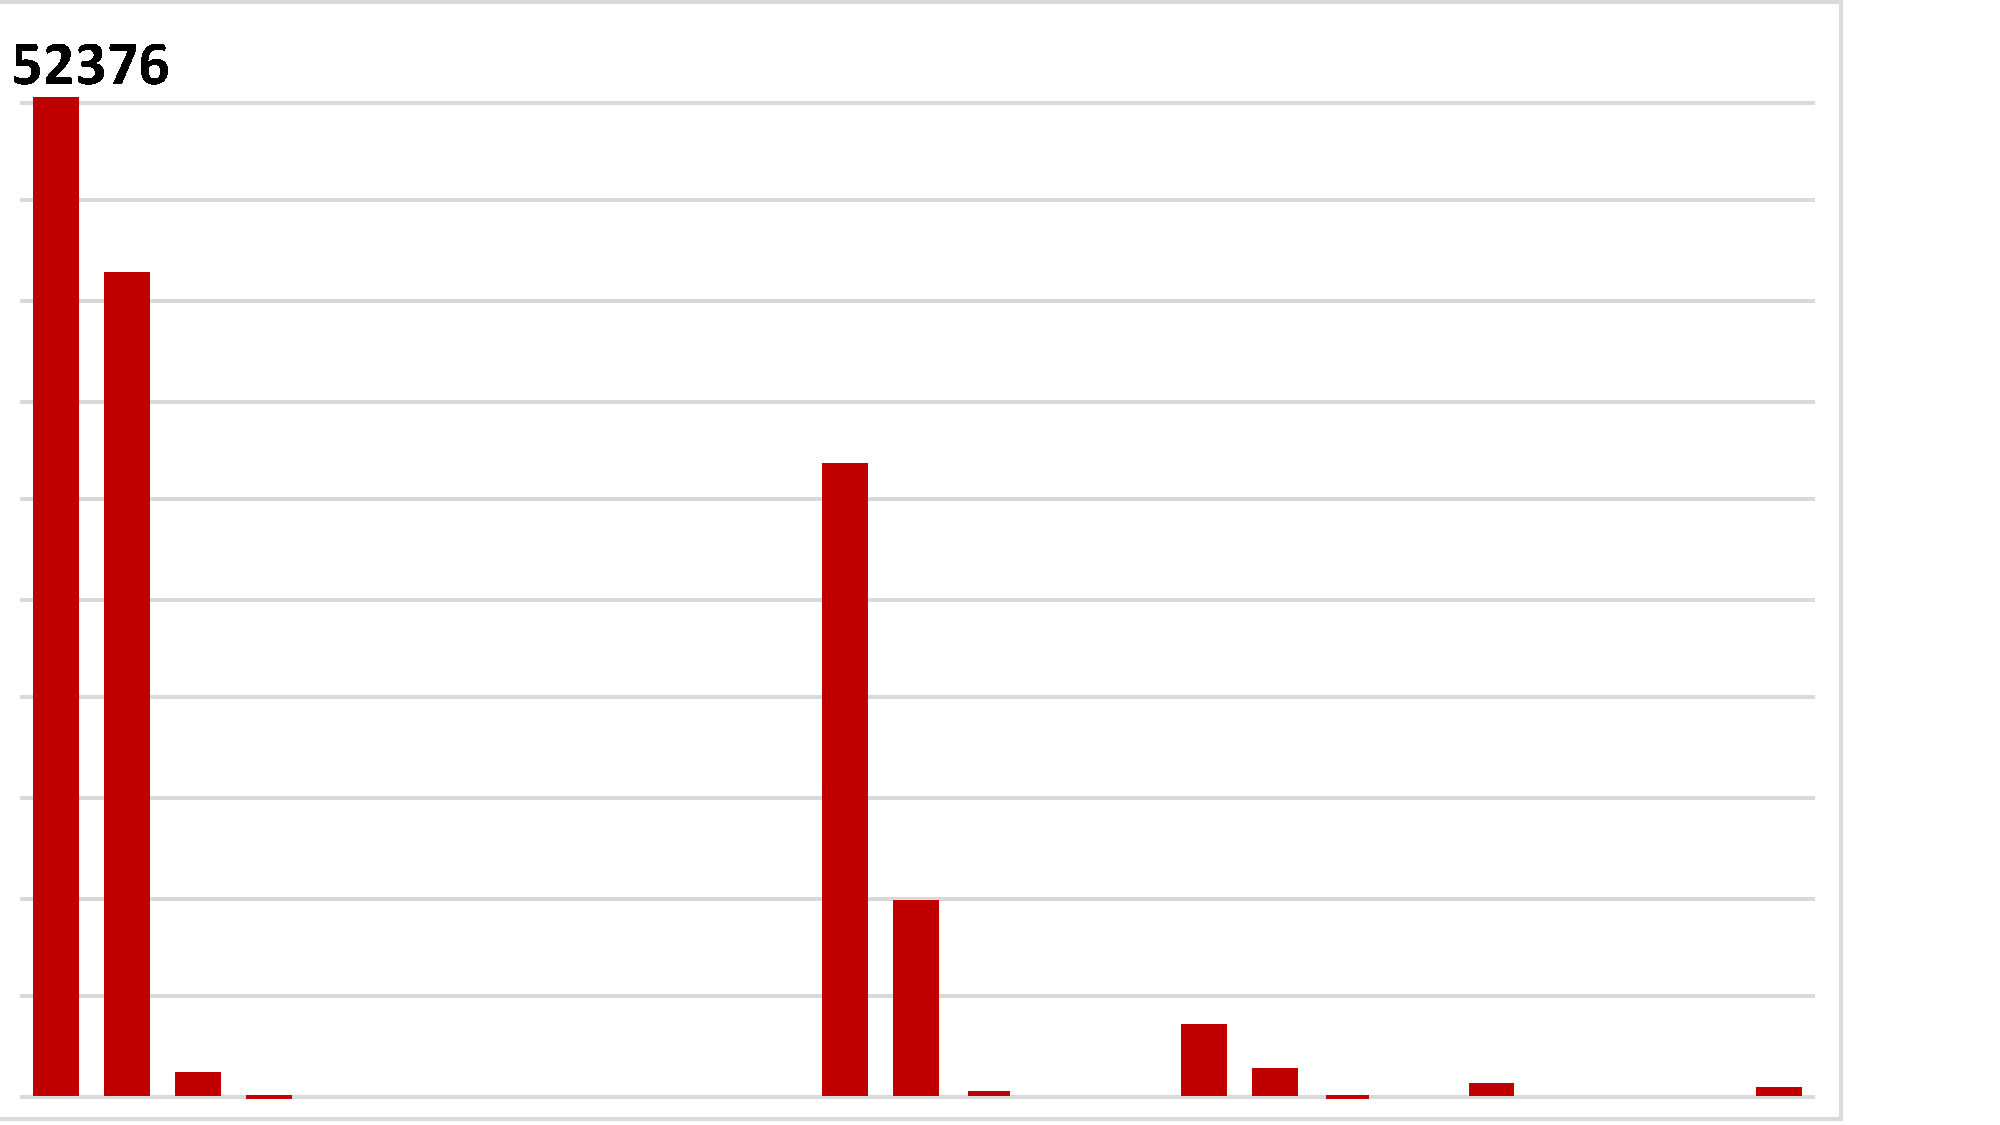
\includegraphics[width=0.95\linewidth, trim={0cm 0cm 2.5cm 0cm}, clip]{results/sw4/Lag3_Max.pdf}
\vspace{-3mm}
\captionof{subfigure}{\footnotesize{Lag 250 1:27 Max$_{L2}$}}
\end{minipage}%
\hfill
\begin{minipage}[t]{0.49\textwidth}%
\centering
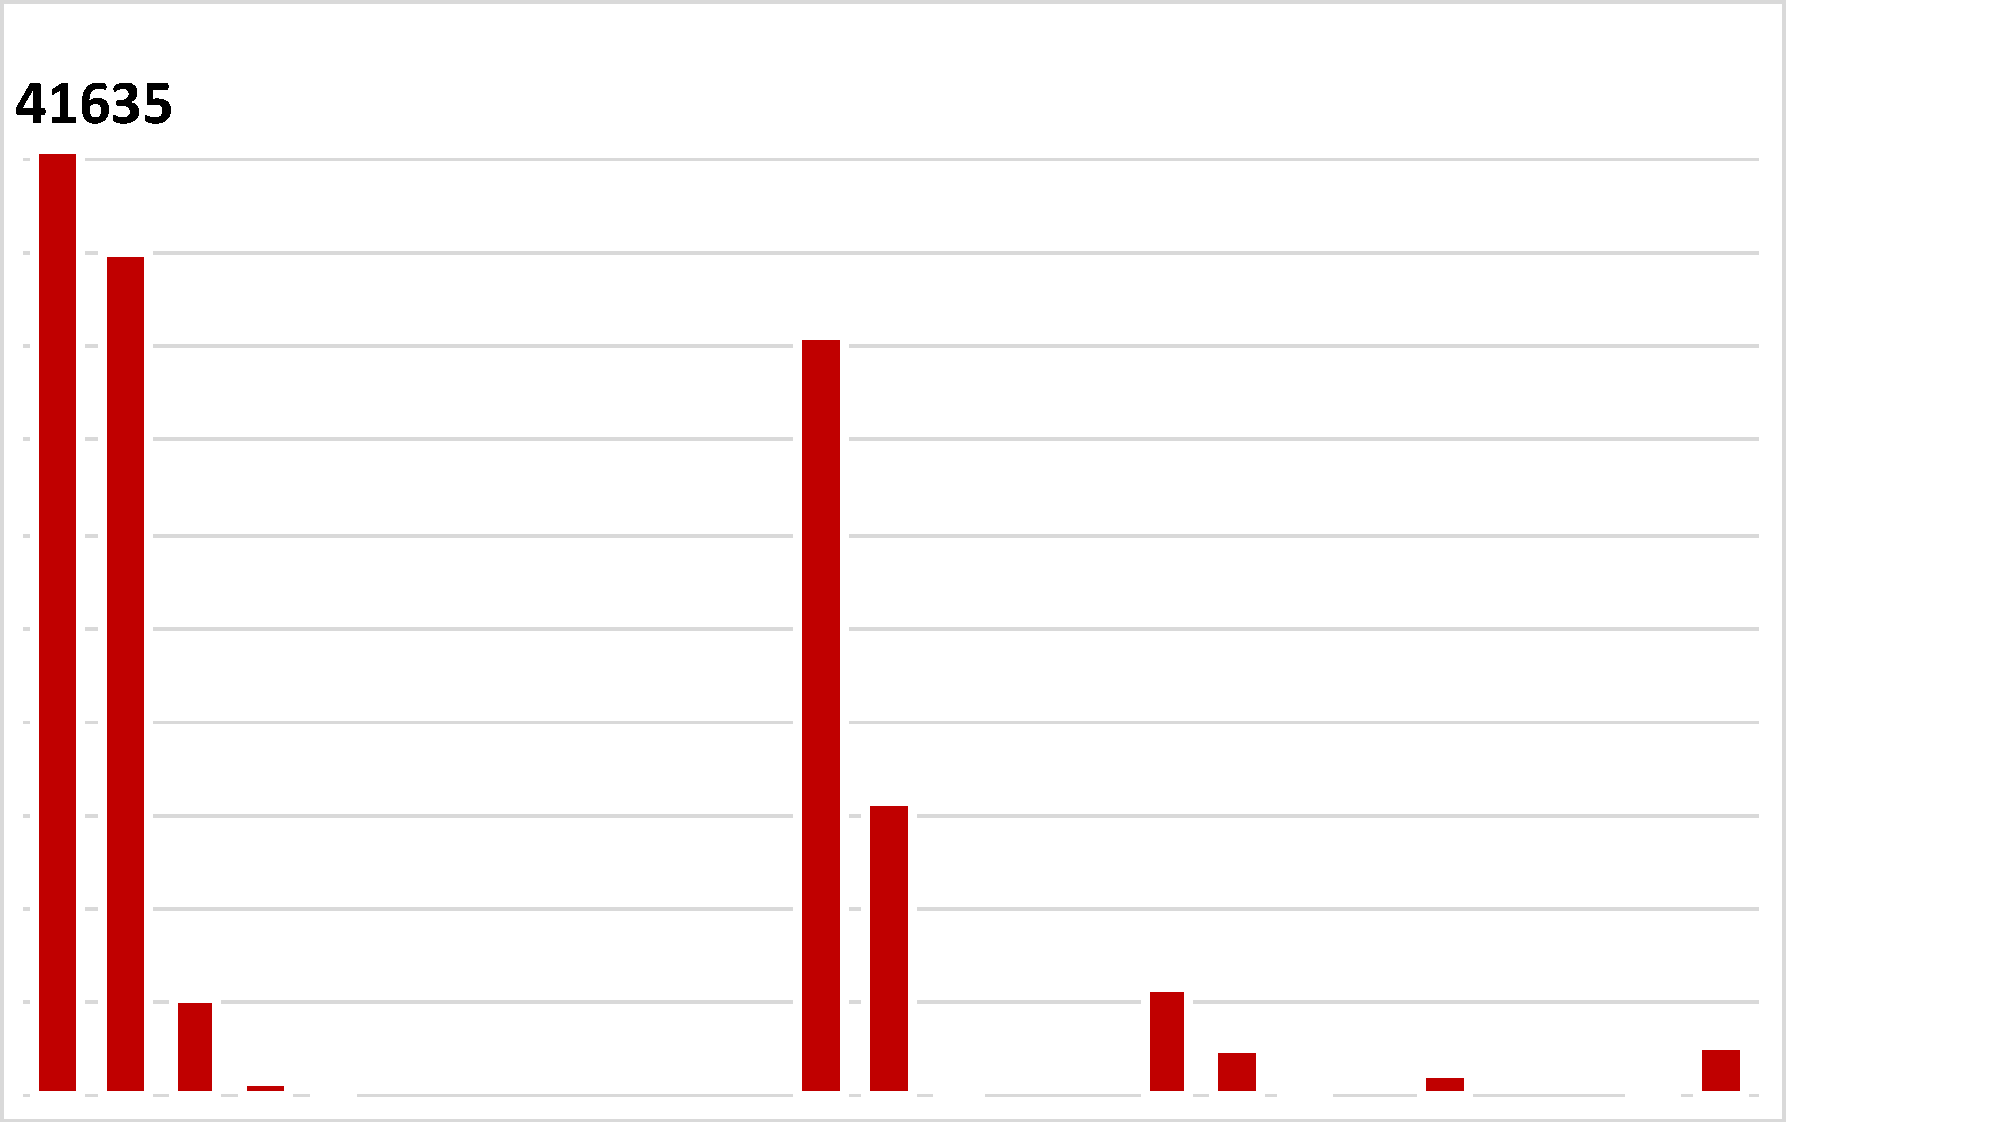
\includegraphics[width=0.95\linewidth, trim={0cm 0cm 2.5cm 0cm}, clip]{results/sw4/Lag4_Max.pdf}
\vspace{-3mm}
\captionof{subfigure}{\footnotesize{Lag 250 1:64 Max$_{L2}$}} 
\end{minipage}
\end{framed}
\vspace{-2mm}
\captionof{figure}{\textbf{SW4} experiment histograms for 90,000 test particle interpolation errors. Each plot has 25 bins, Eulerian bins range from $<$0.6 to $>$15, Lagrangian bins range from 0 to $>$0.2, with bar height encoding number of particles. Horizontal grid lines mark increments of 2,000.}
\label{fig:sw4_histograms}
\end{minipage}% End of SW4
%%%%%%%%%%%%%%%%%%%%%%%%%%%%%%%%%%%
\setcounter{subfigure}{0}
\hfill
\begin{minipage}[t]{0.66\linewidth}%
\begin{framed}
\begin{minipage}[t]{0.24\textwidth}%
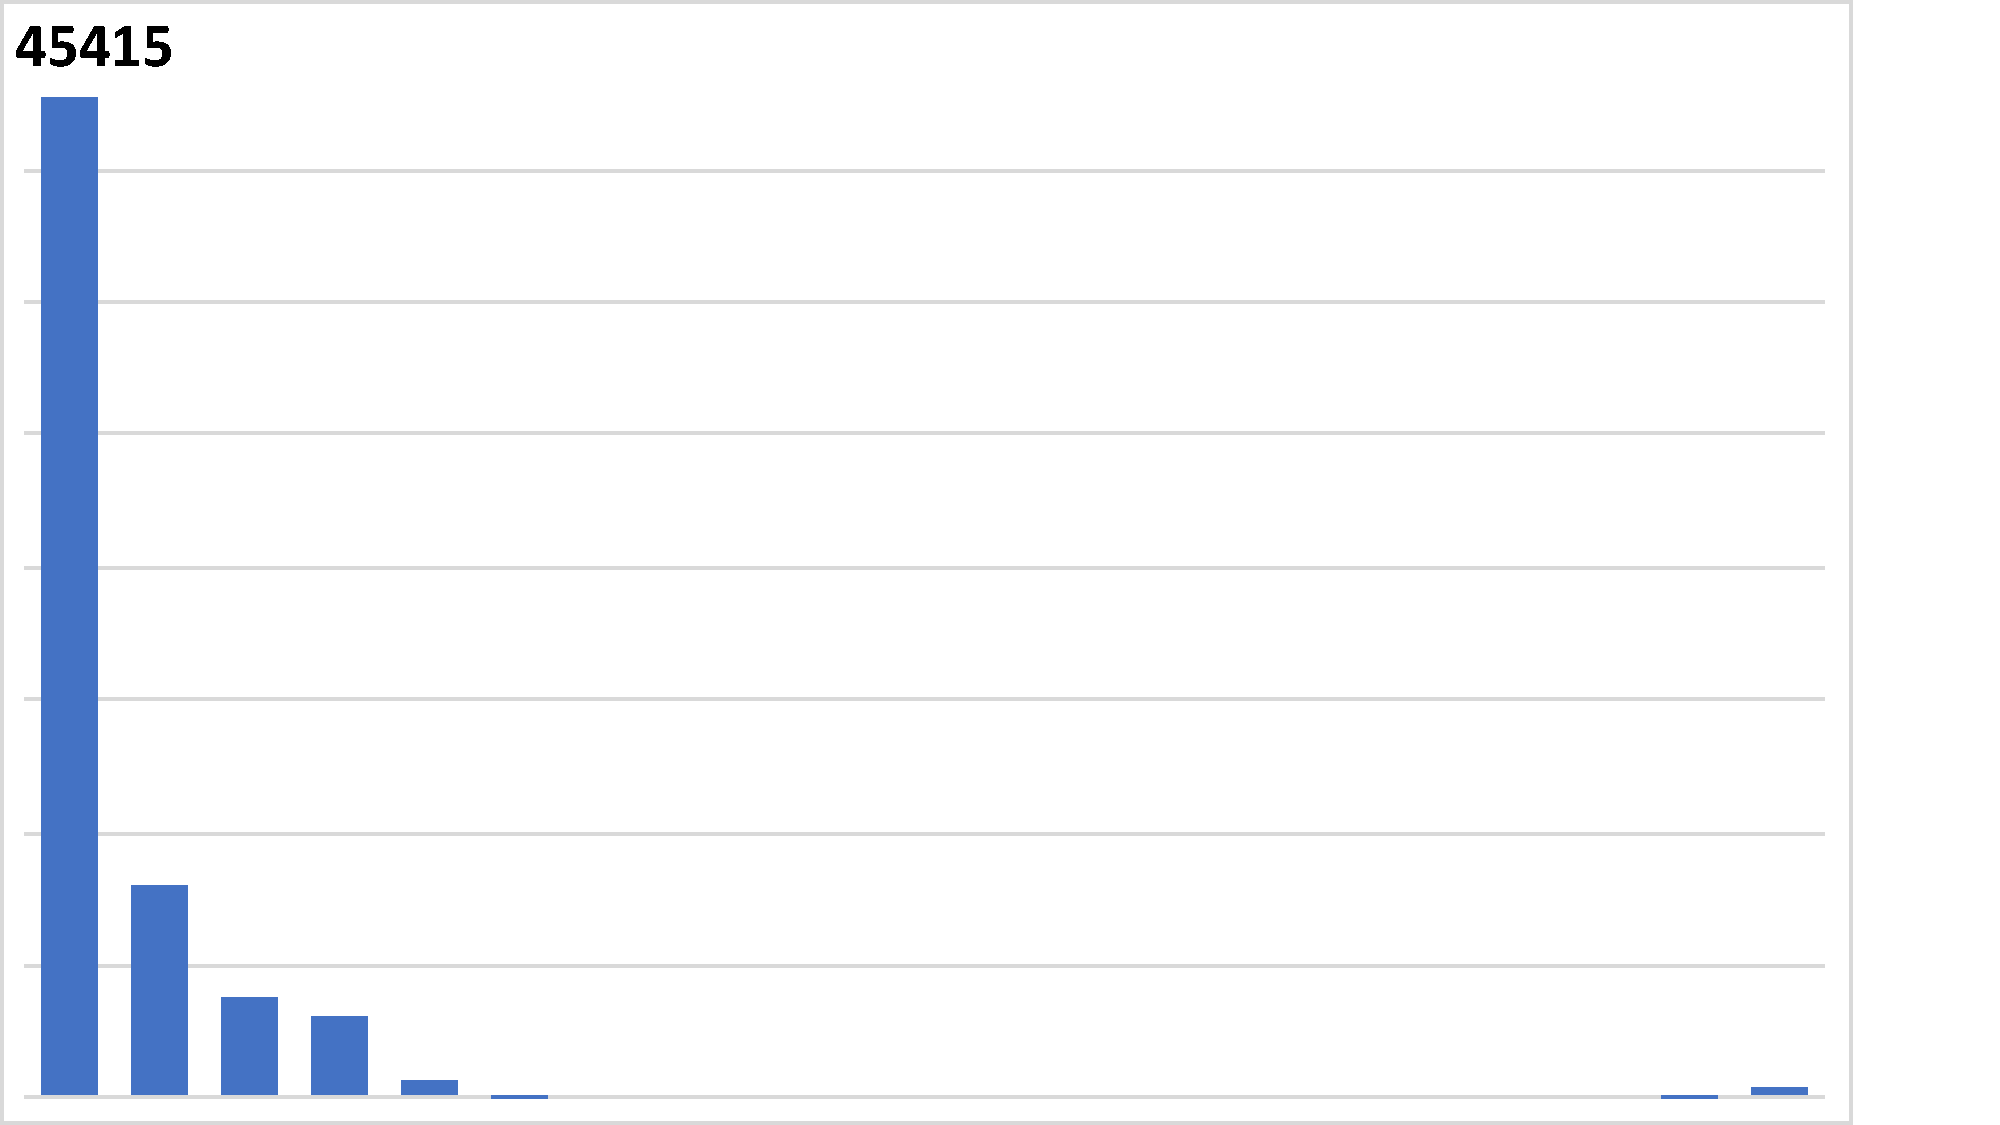
\includegraphics[width=0.95\linewidth, trim={0cm 0cm 2.5cm 0cm}, clip]{results/nyx/Eul25_AvgL2.pdf}
\vspace{-2mm}
\captionof{subfigure}{Eul 25 Avg$_{L2}$}
\end{minipage}%
\hfill
\begin{minipage}[t]{0.24\textwidth}%
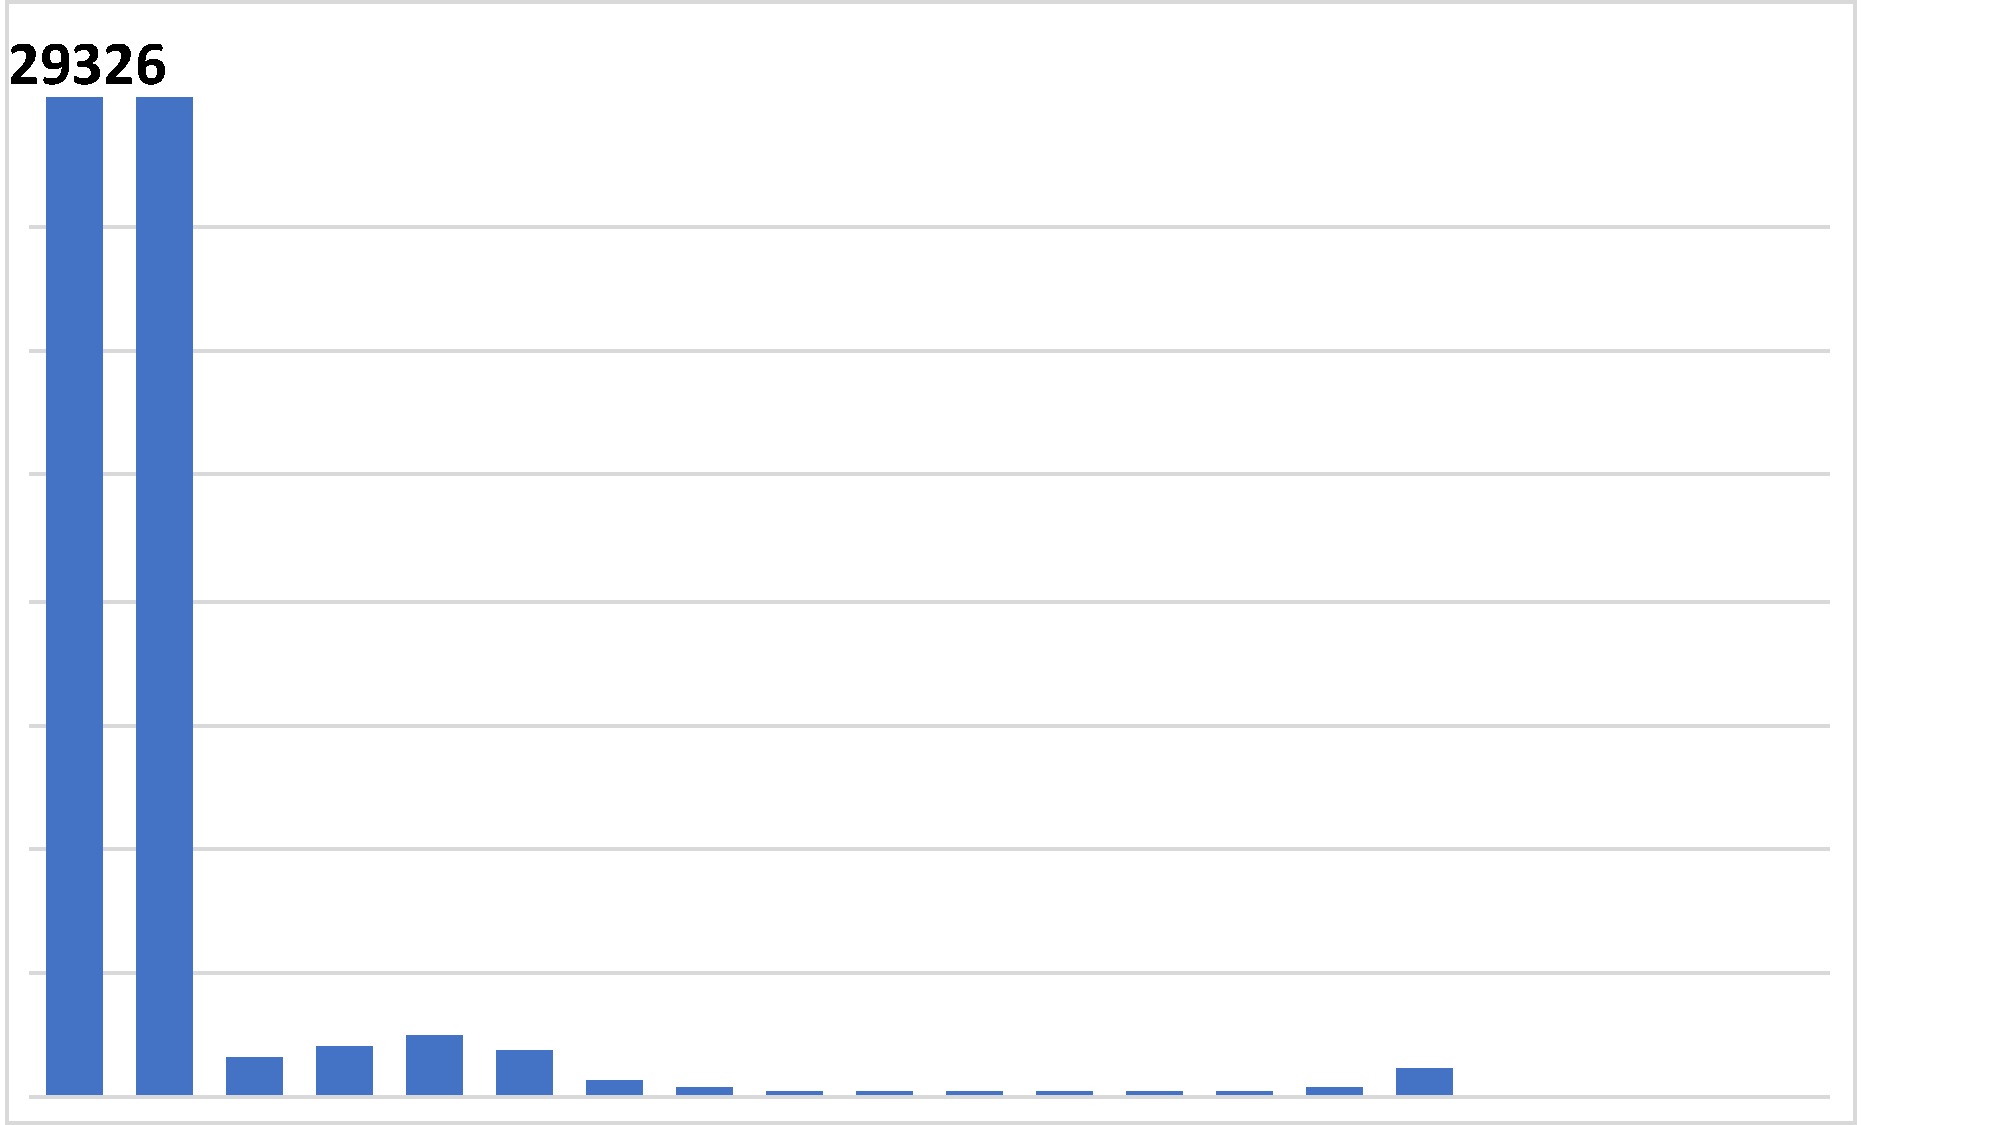
\includegraphics[width=0.95\linewidth, trim={0cm 0cm 2.5cm 0cm}, clip]{results/nyx/Eul50_AvgL2.pdf}
\vspace{-2mm}
\captionof{subfigure}{Eul 50 Avg$_{L2}$}
\end{minipage}
\begin{minipage}[t]{0.24\textwidth}%
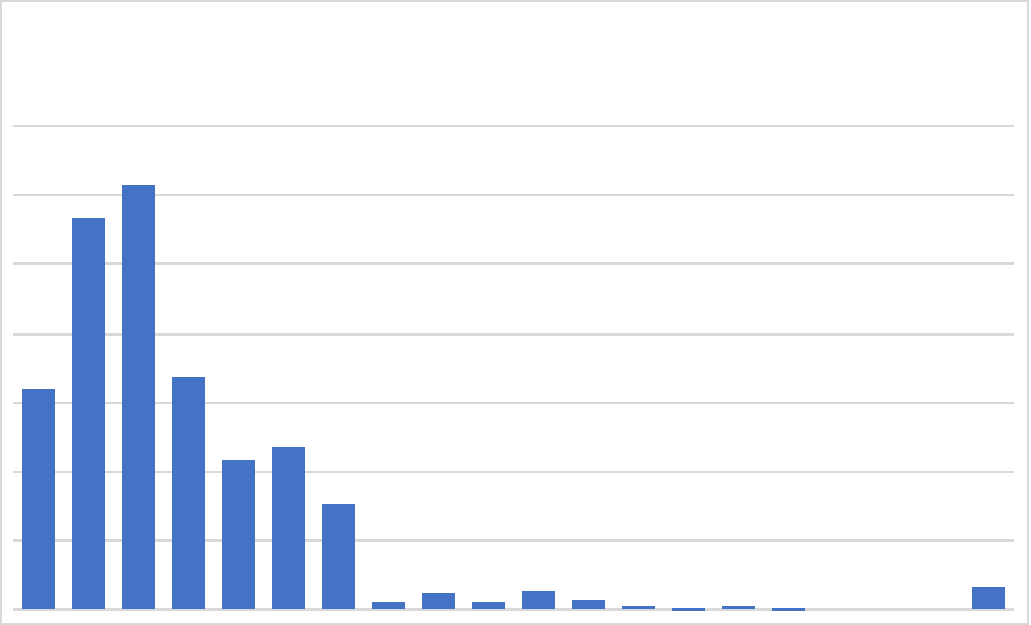
\includegraphics[width=0.95\linewidth]{results/nyx/Eul100_AvgL2.pdf}
\vspace{-2mm}
\captionof{subfigure}{Eul 100 Avg$_{L2}$}
\end{minipage}%
\hfill
\begin{minipage}[t]{0.24\textwidth}%
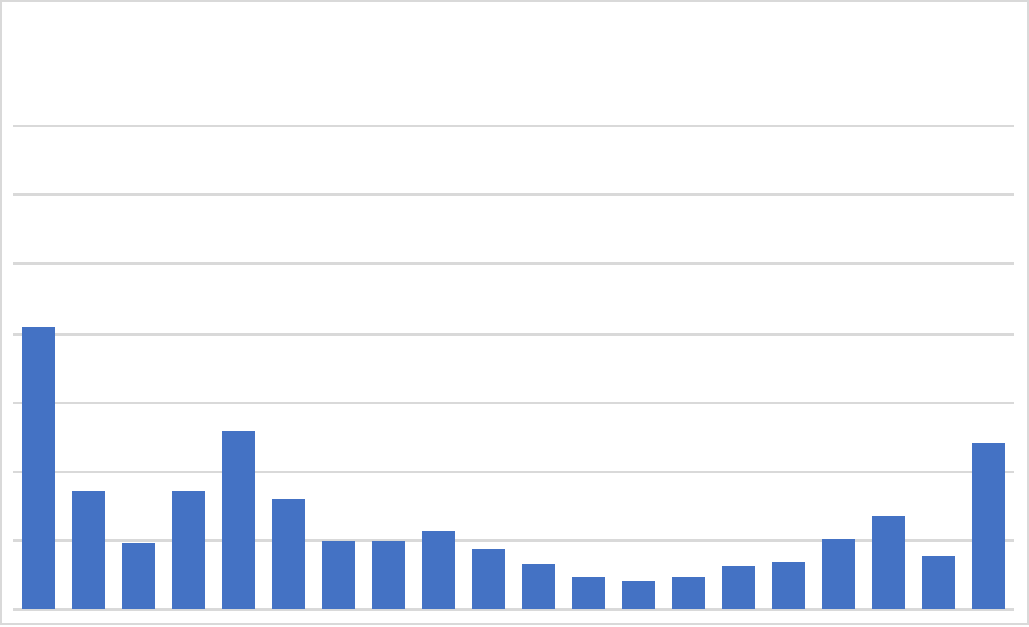
\includegraphics[width=0.95\linewidth]{results/nyx/Eul200_AvgL2.pdf}
\vspace{-2mm}
\captionof{subfigure}{Eul 200 Avg$_{L2}$}
\end{minipage}
\begin{minipage}[t]{0.24\textwidth}%
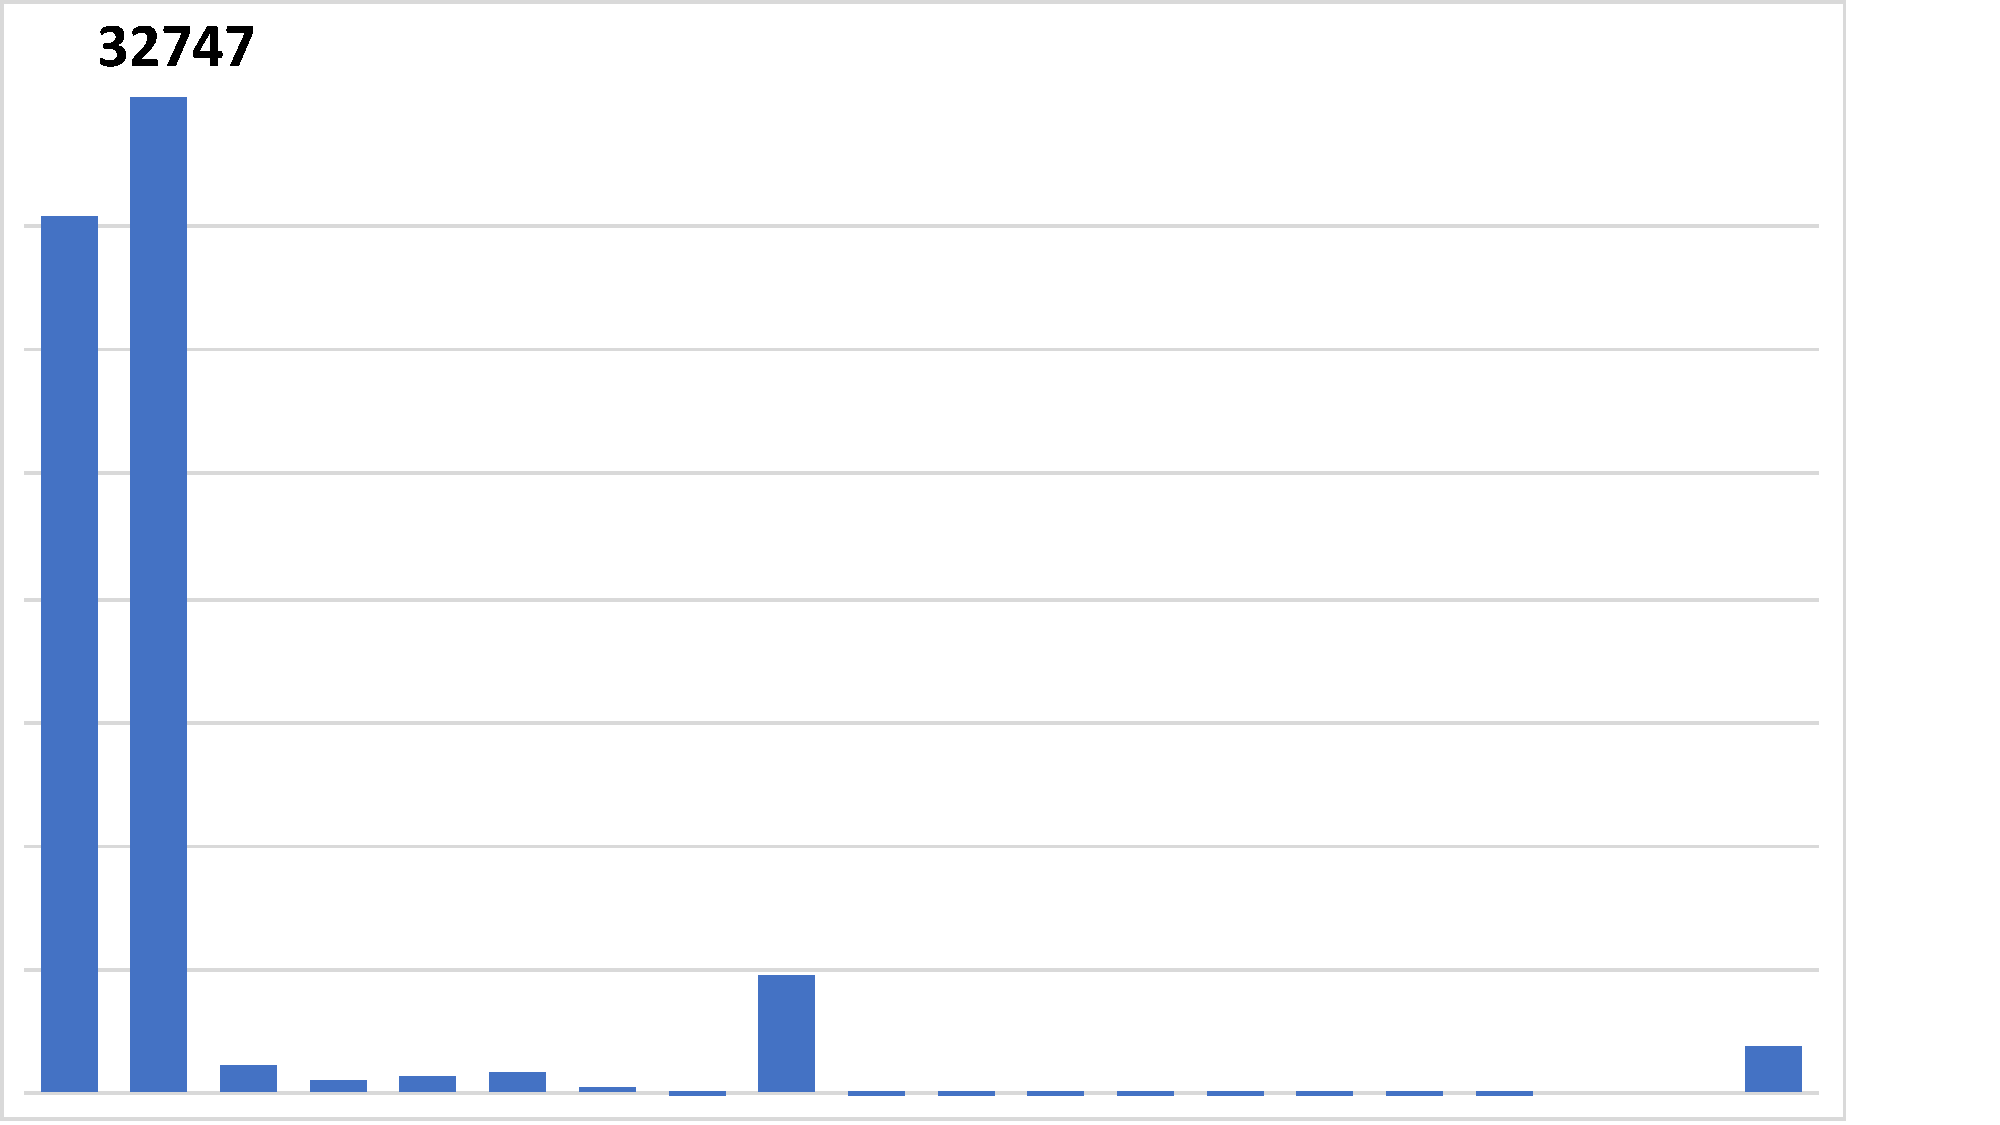
\includegraphics[width=0.95\linewidth, trim={0cm 0cm 2.5cm 0cm}, clip]{results/nyx/Eul25_Max.pdf}
\vspace{-2mm}
\captionof{subfigure}{Eul 25 Max$_{L2}$}
\end{minipage}%
\hfill
\begin{minipage}[t]{0.24\textwidth}%
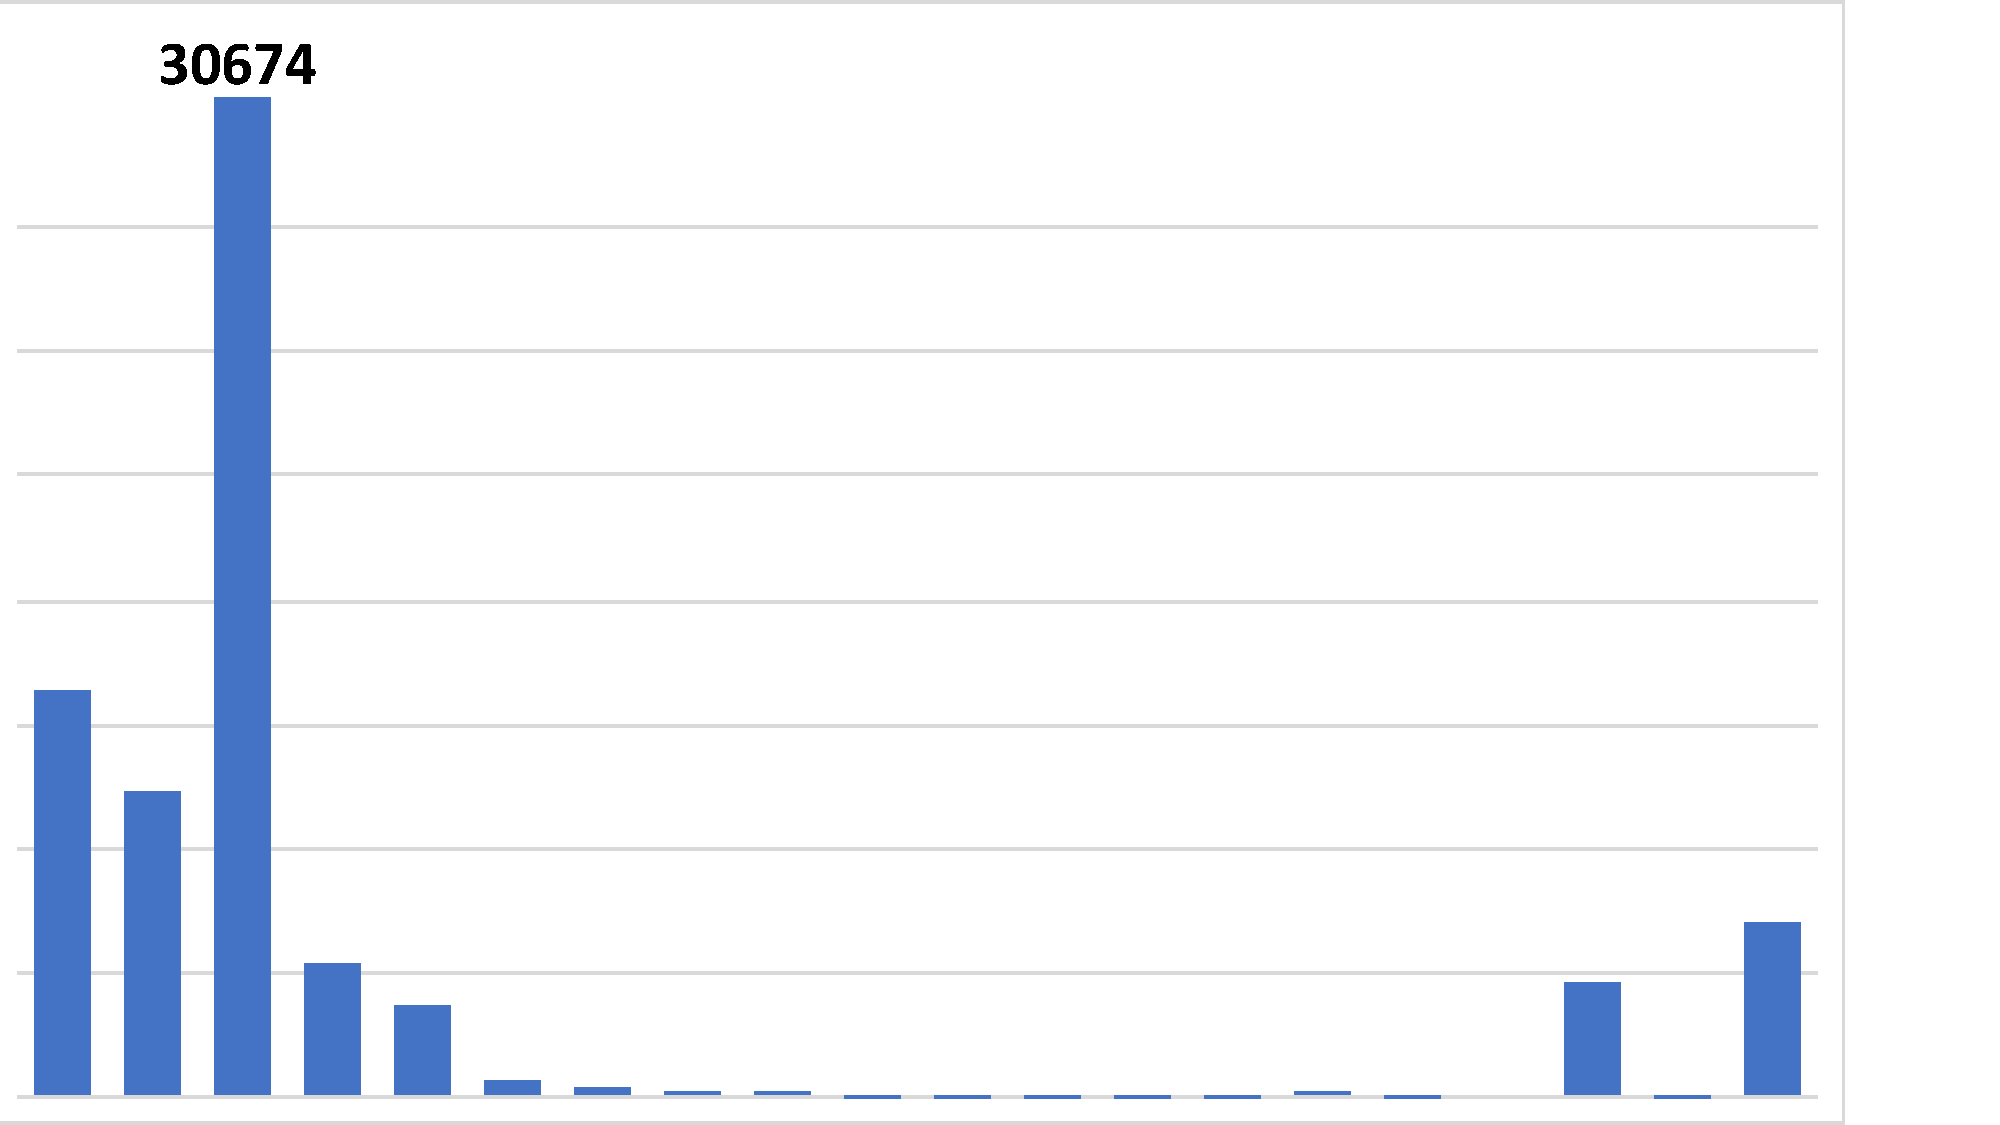
\includegraphics[width=0.95\linewidth, trim={0cm 0cm 2.5cm 0cm}, clip]{results/nyx/Eul50_Max.pdf}
\vspace{-2mm}
\captionof{subfigure}{Eul 50 Max$_{L2}$}
\end{minipage}
\begin{minipage}[t]{0.24\textwidth}%
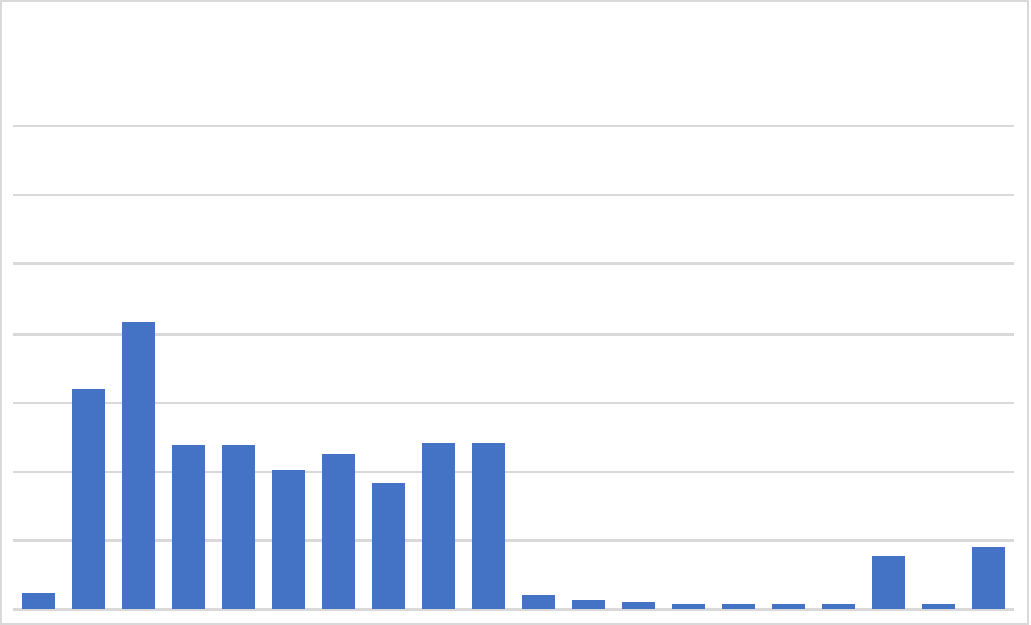
\includegraphics[width=0.95\linewidth]{results/nyx/Eul100_Max.pdf}
\vspace{-2mm}
\captionof{subfigure}{Eul 100 Max$_{L2}$}
\end{minipage}%
\hfill
\begin{minipage}[t]{0.24\textwidth}%
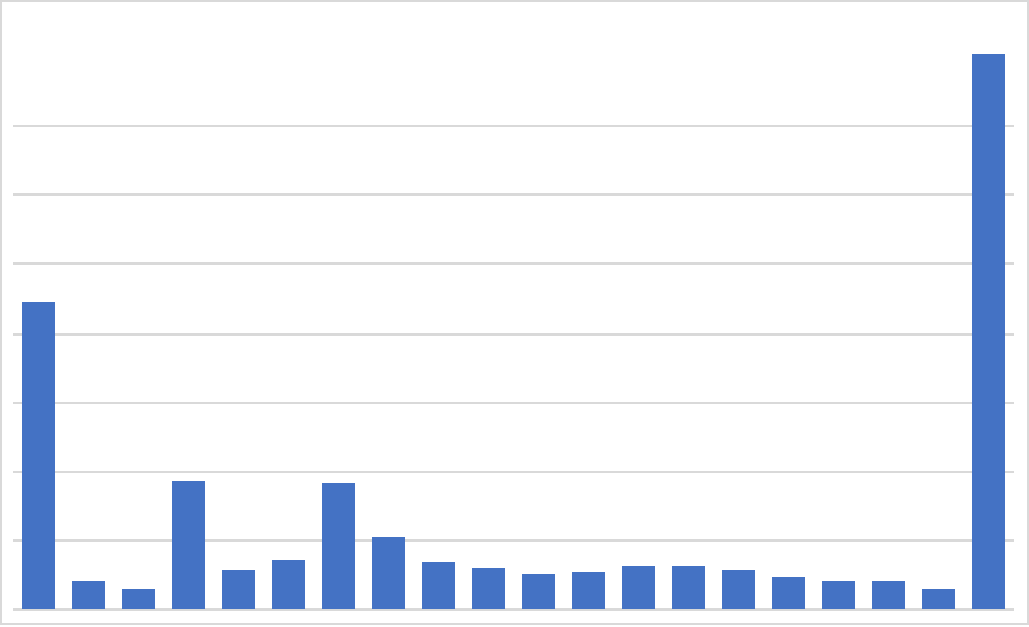
\includegraphics[width=0.95\linewidth]{results/nyx/Eul200_Max.pdf}
\vspace{-2mm}
\captionof{subfigure}{Eul 200 Max$_{L2}$}
\end{minipage}
%%%% Begin Nyx Lagrangian %%% 
\begin{minipage}[t]{0.24\textwidth}%
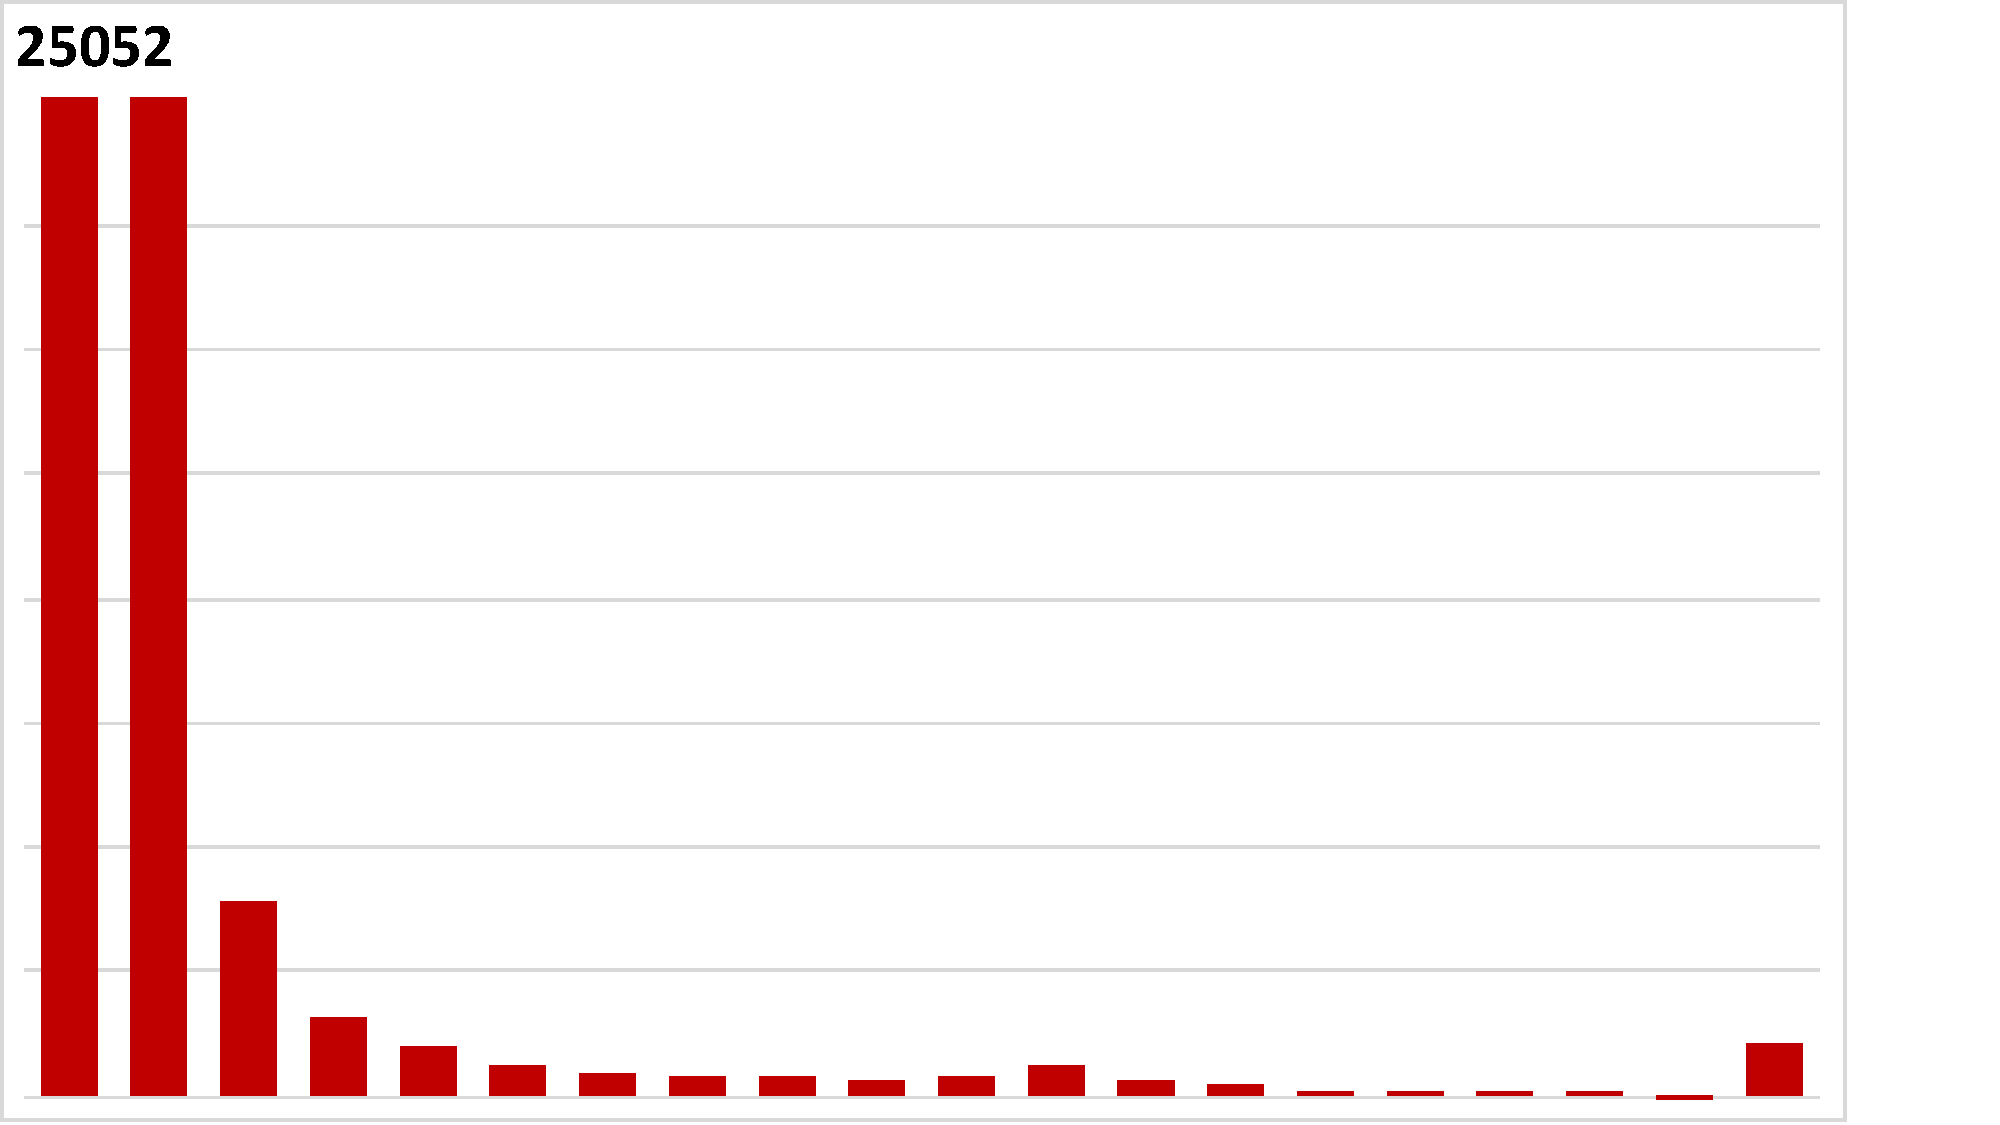
\includegraphics[width=0.95\linewidth, trim={0cm 0cm 2.5cm 0cm}, clip]{results/nyx/Lag25_1_AvgL2.pdf}
\vspace{-2mm}
\captionof{subfigure}{Lag 25 Avg$_{L2}$}
\end{minipage}%
\hfill
\begin{minipage}[t]{0.24\textwidth}%
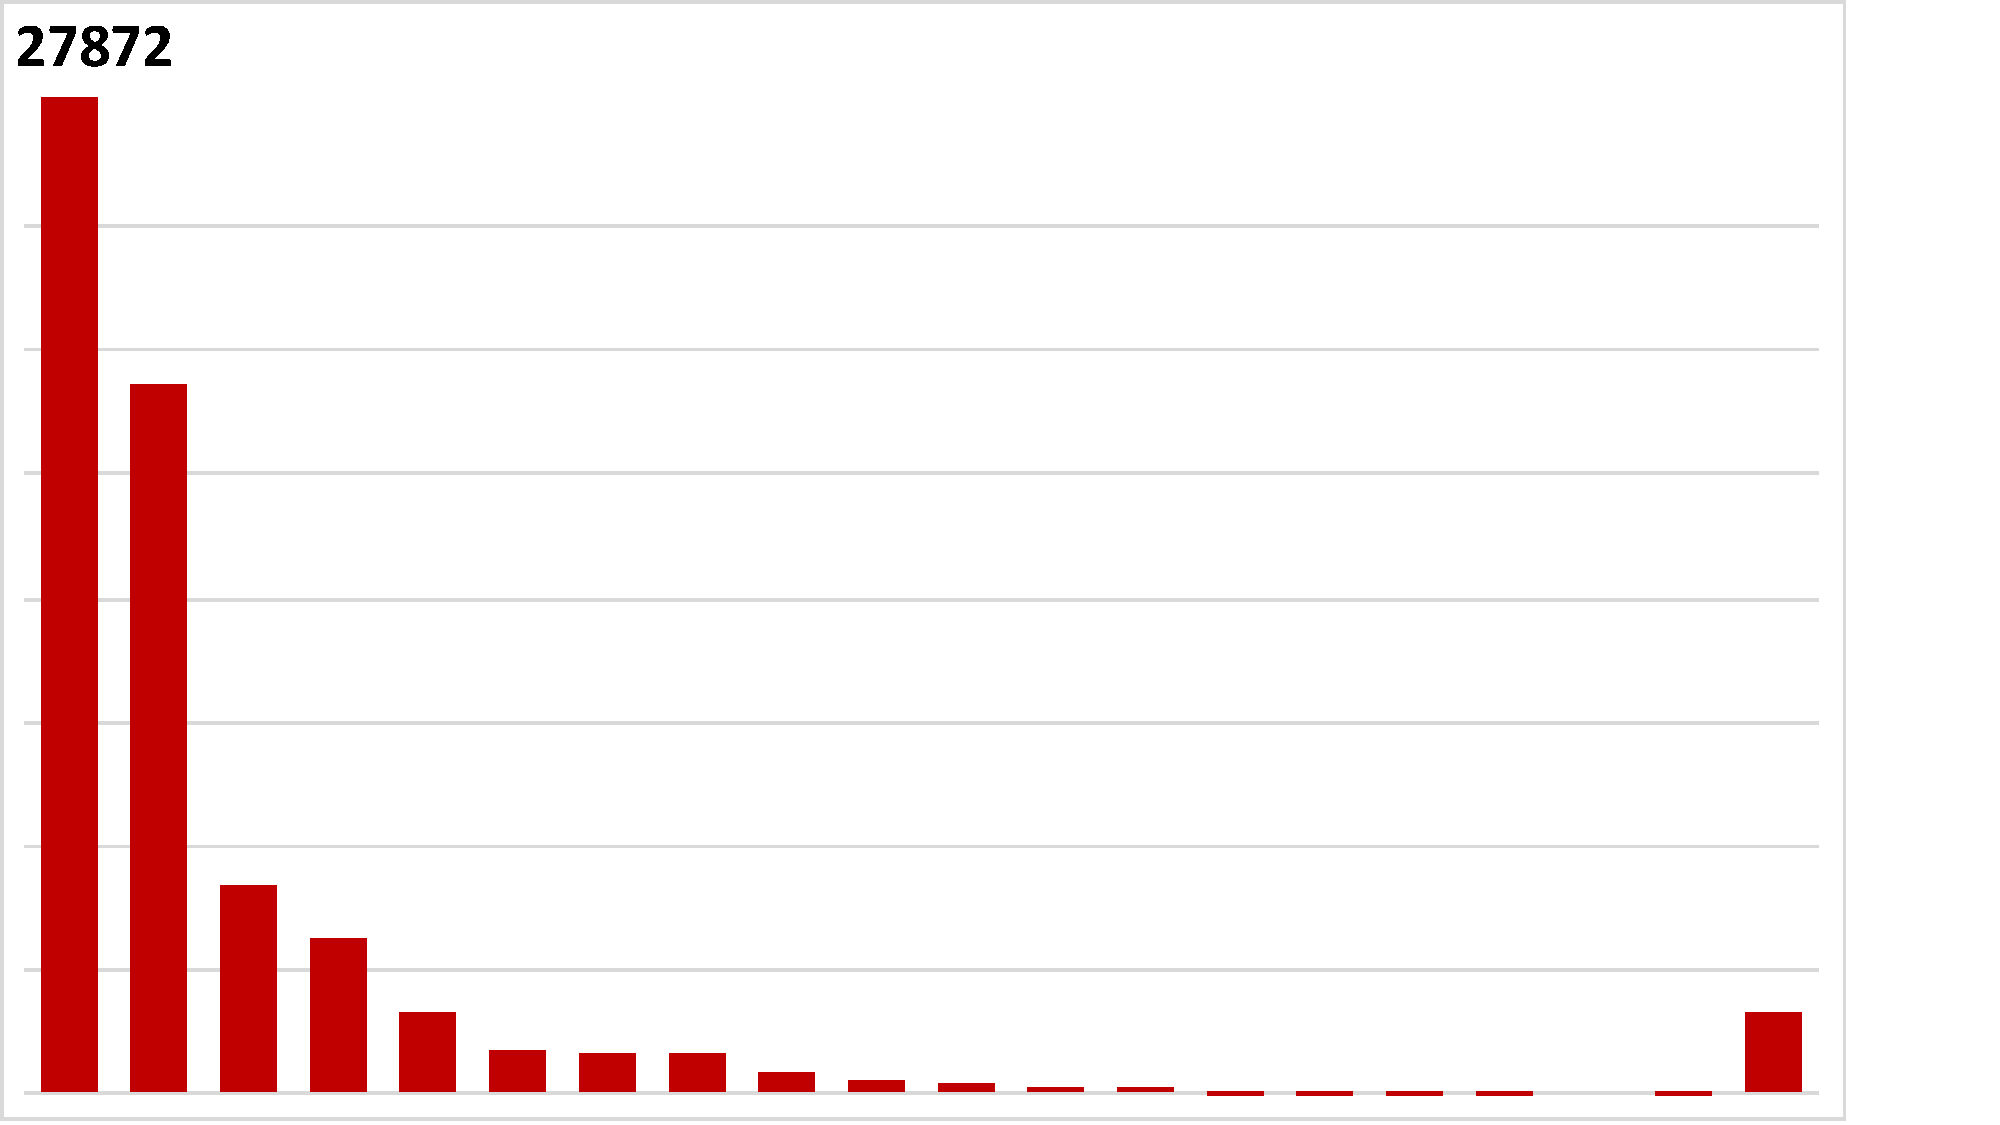
\includegraphics[width=0.95\linewidth, trim={0cm 0cm 2.5cm 0cm}, clip]{results/nyx/Lag50_1_AvgL2.pdf}
\vspace{-2mm}
\captionof{subfigure}{Lag 50 Avg$_{L2}$}
\end{minipage}
\begin{minipage}[t]{0.24\textwidth}%
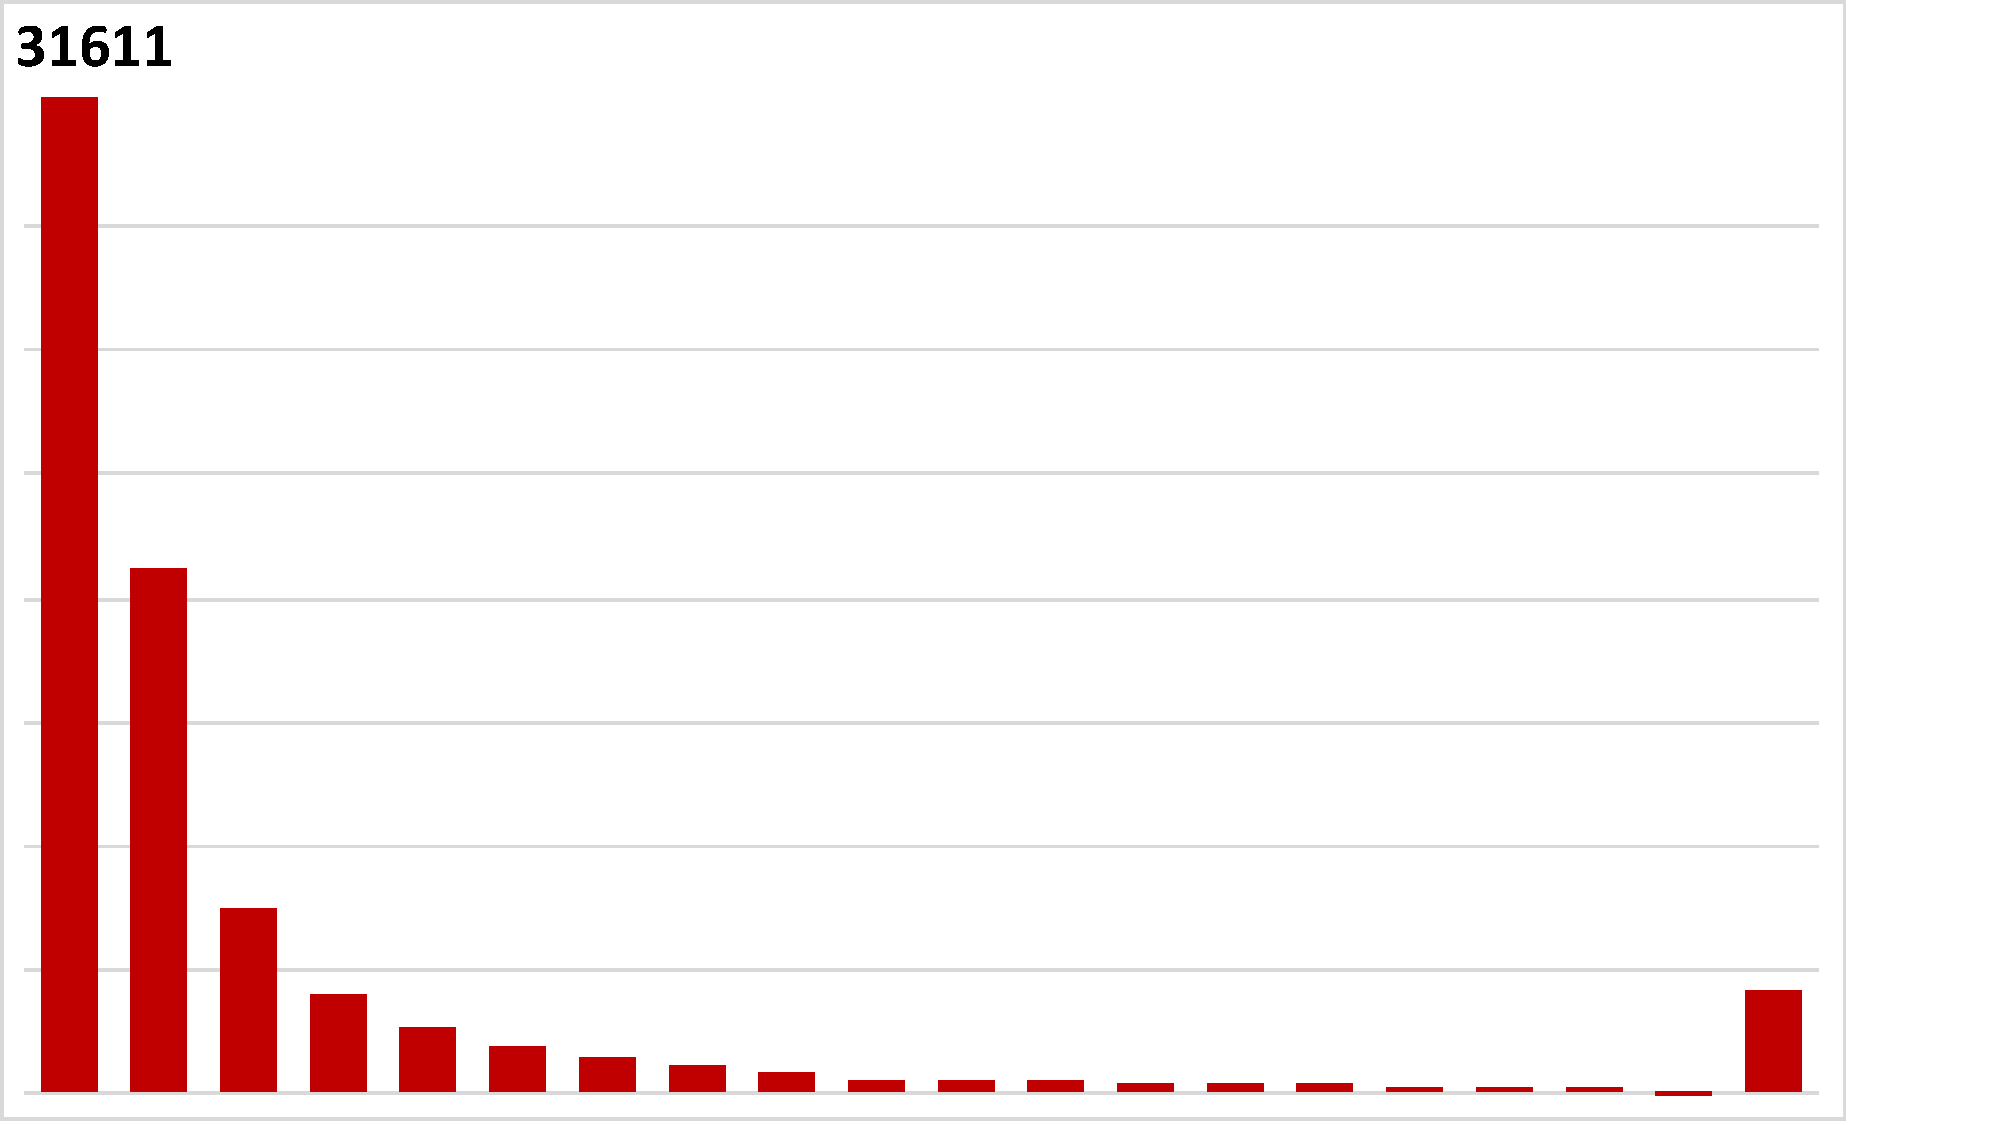
\includegraphics[width=0.95\linewidth, trim={0cm 0cm 2.5cm 0cm}, clip]{results/nyx/Lag100_1_AvgL2.pdf}
\vspace{-2mm}
\captionof{subfigure}{Lag 100 Avg$_{L2}$}
\end{minipage}%
\hfill
\begin{minipage}[t]{0.24\textwidth}%
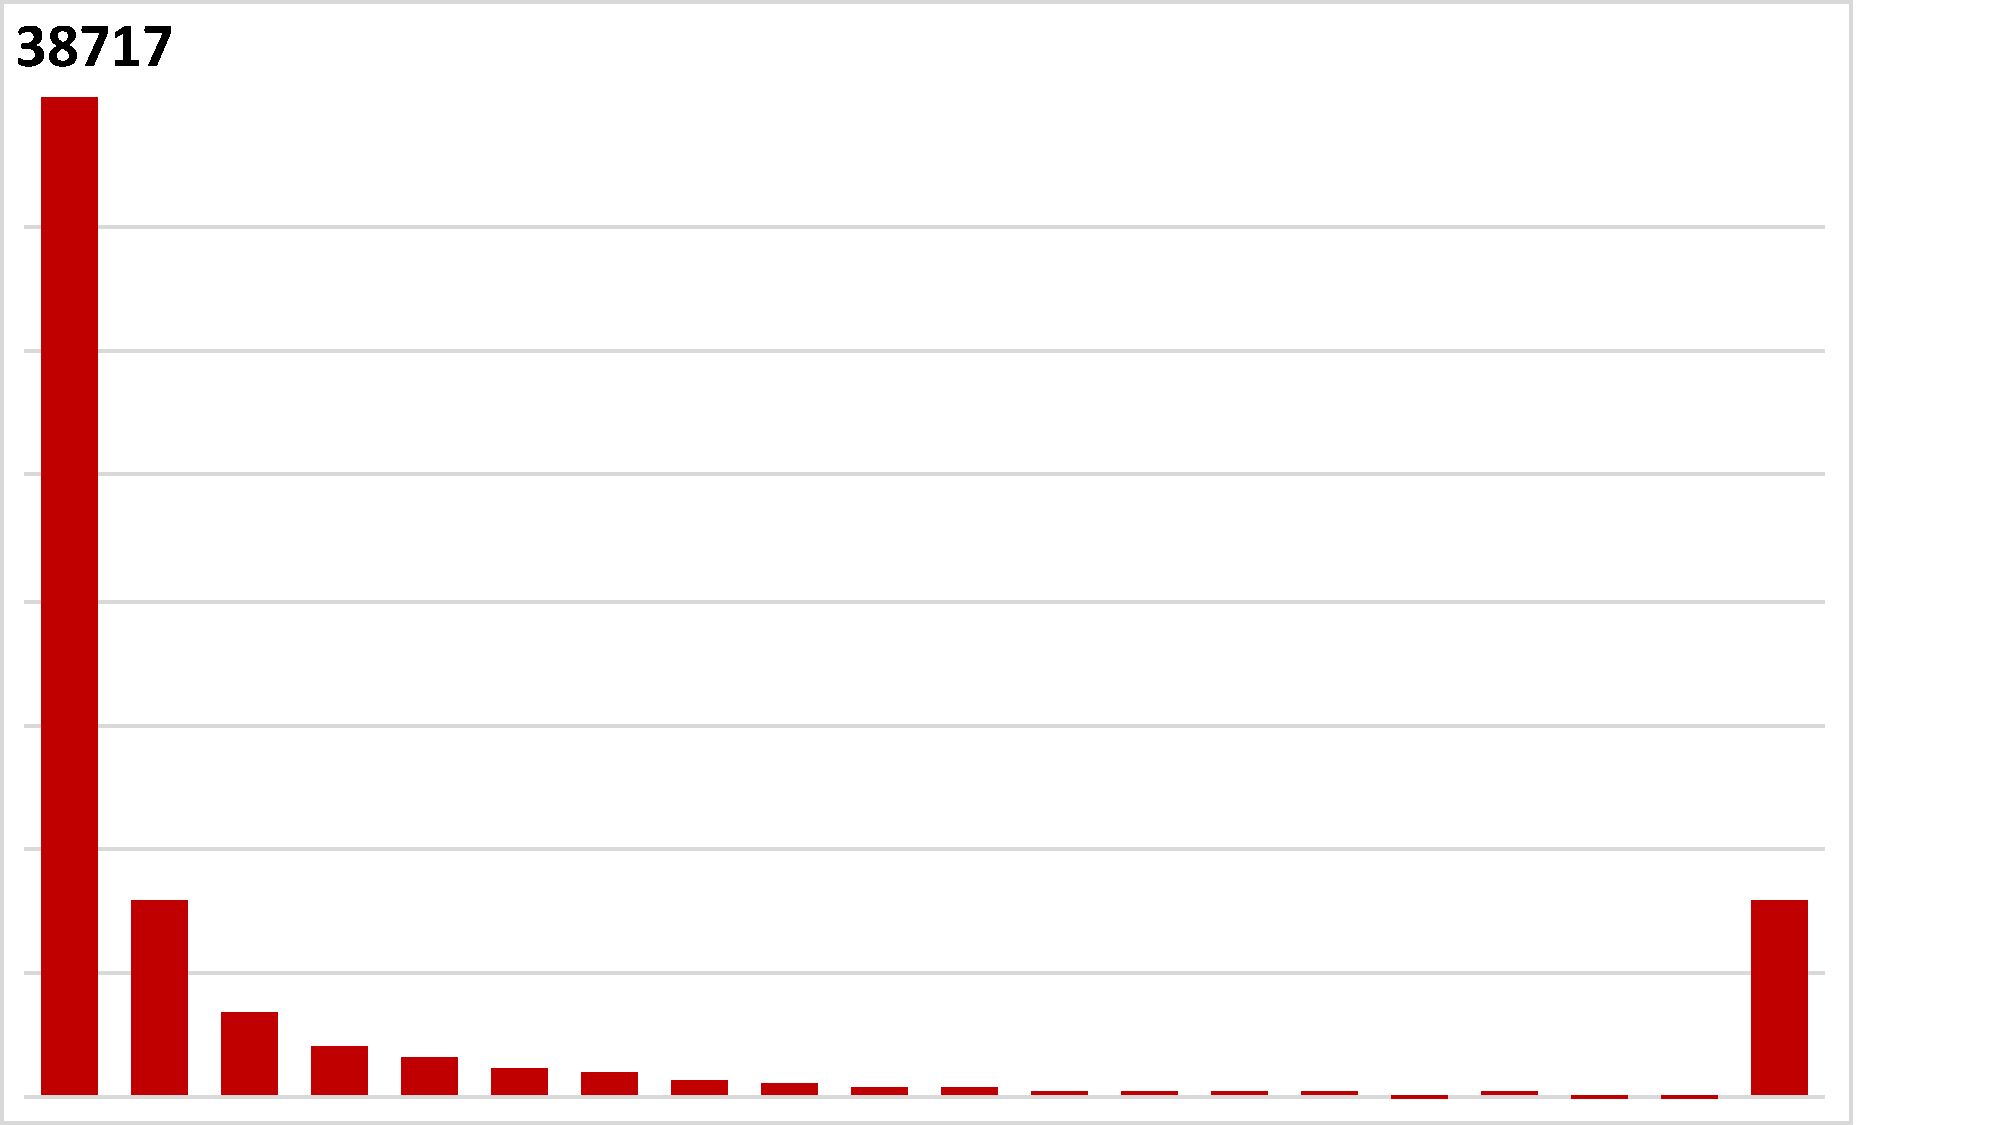
\includegraphics[width=0.95\linewidth, trim={0cm 0cm 2.5cm 0cm}, clip]{results/nyx/Lag200_1_AvgL2.pdf}
\vspace{-2mm}
\captionof{subfigure}{Lag 200 Avg$_{L2}$}
\end{minipage}
\begin{minipage}[t]{0.24\textwidth}%
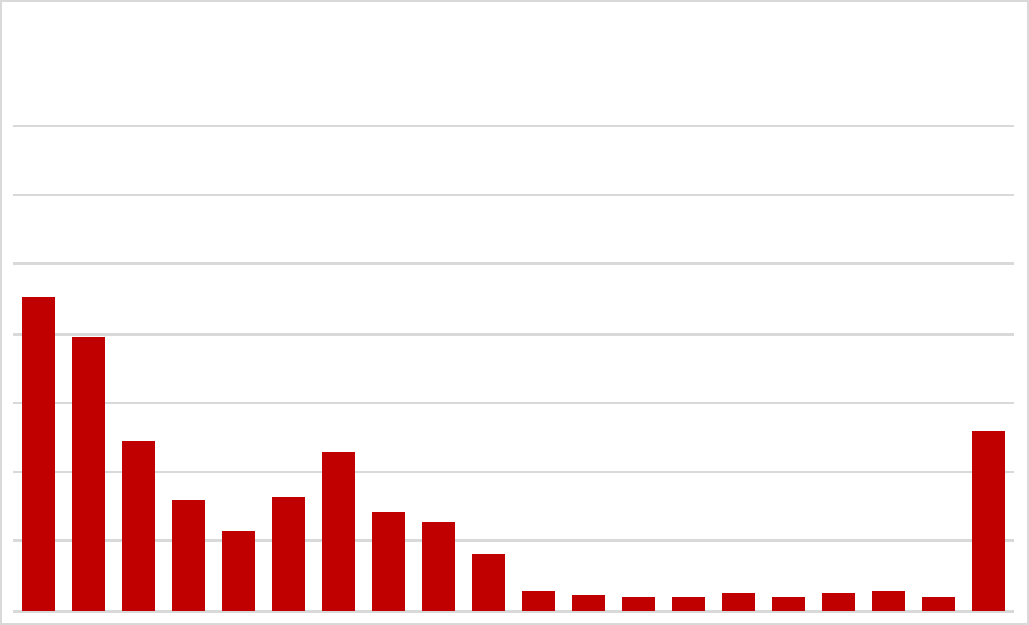
\includegraphics[width=0.95\linewidth, trim={0cm 0cm 2.5cm 0cm}, clip]{results/nyx/Lag25_1_Max.pdf}
\vspace{-2mm}
\captionof{subfigure}{Lag 25 Max$_{L2}$}
\end{minipage}%
\hfill
\begin{minipage}[t]{0.24\textwidth}%
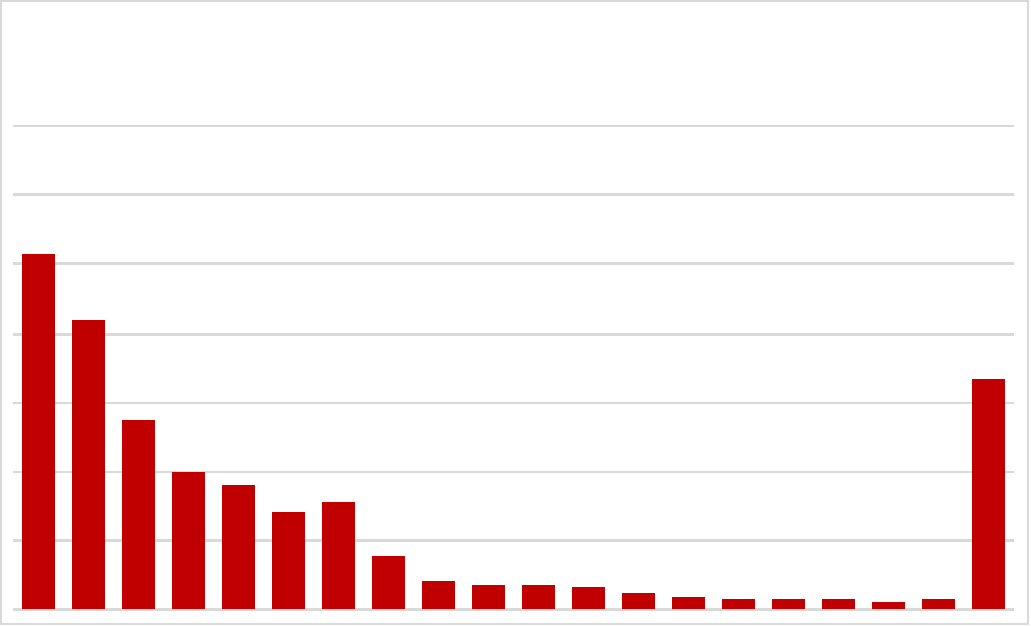
\includegraphics[width=0.95\linewidth, trim={0cm 0cm 2.5cm 0cm}, clip]{results/nyx/Lag50_1_Max.pdf}
\vspace{-2mm}
\captionof{subfigure}{Lag 50 Max$_{L2}$}
\end{minipage}
\begin{minipage}[t]{0.24\textwidth}%
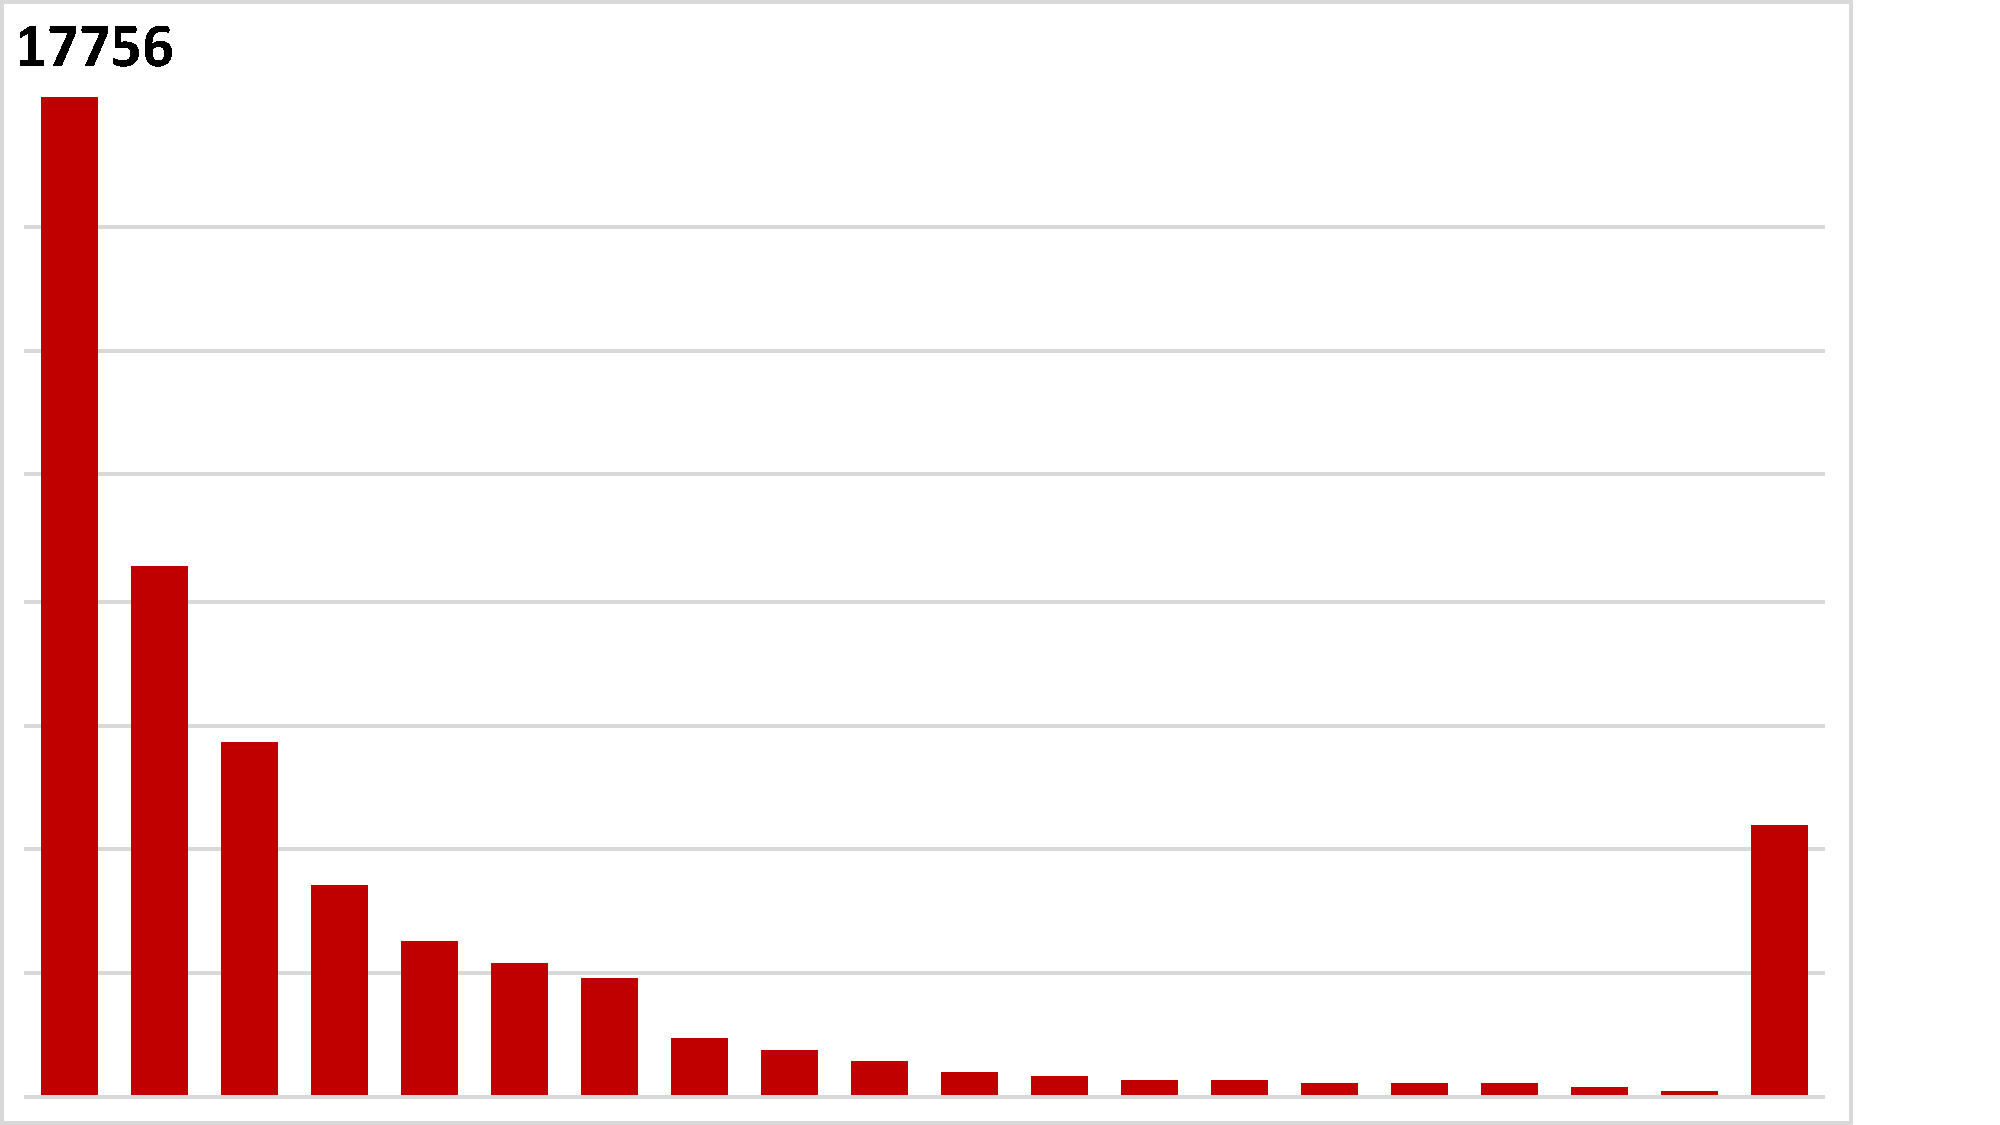
\includegraphics[width=0.95\linewidth, trim={0cm 0cm 2.5cm 0cm}, clip]{results/nyx/Lag100_1_Max.pdf}
\vspace{-2mm}
\captionof{subfigure}{Lag 100 Max$_{L2}$}
\end{minipage}%
\hfill
\begin{minipage}[t]{0.24\textwidth}%
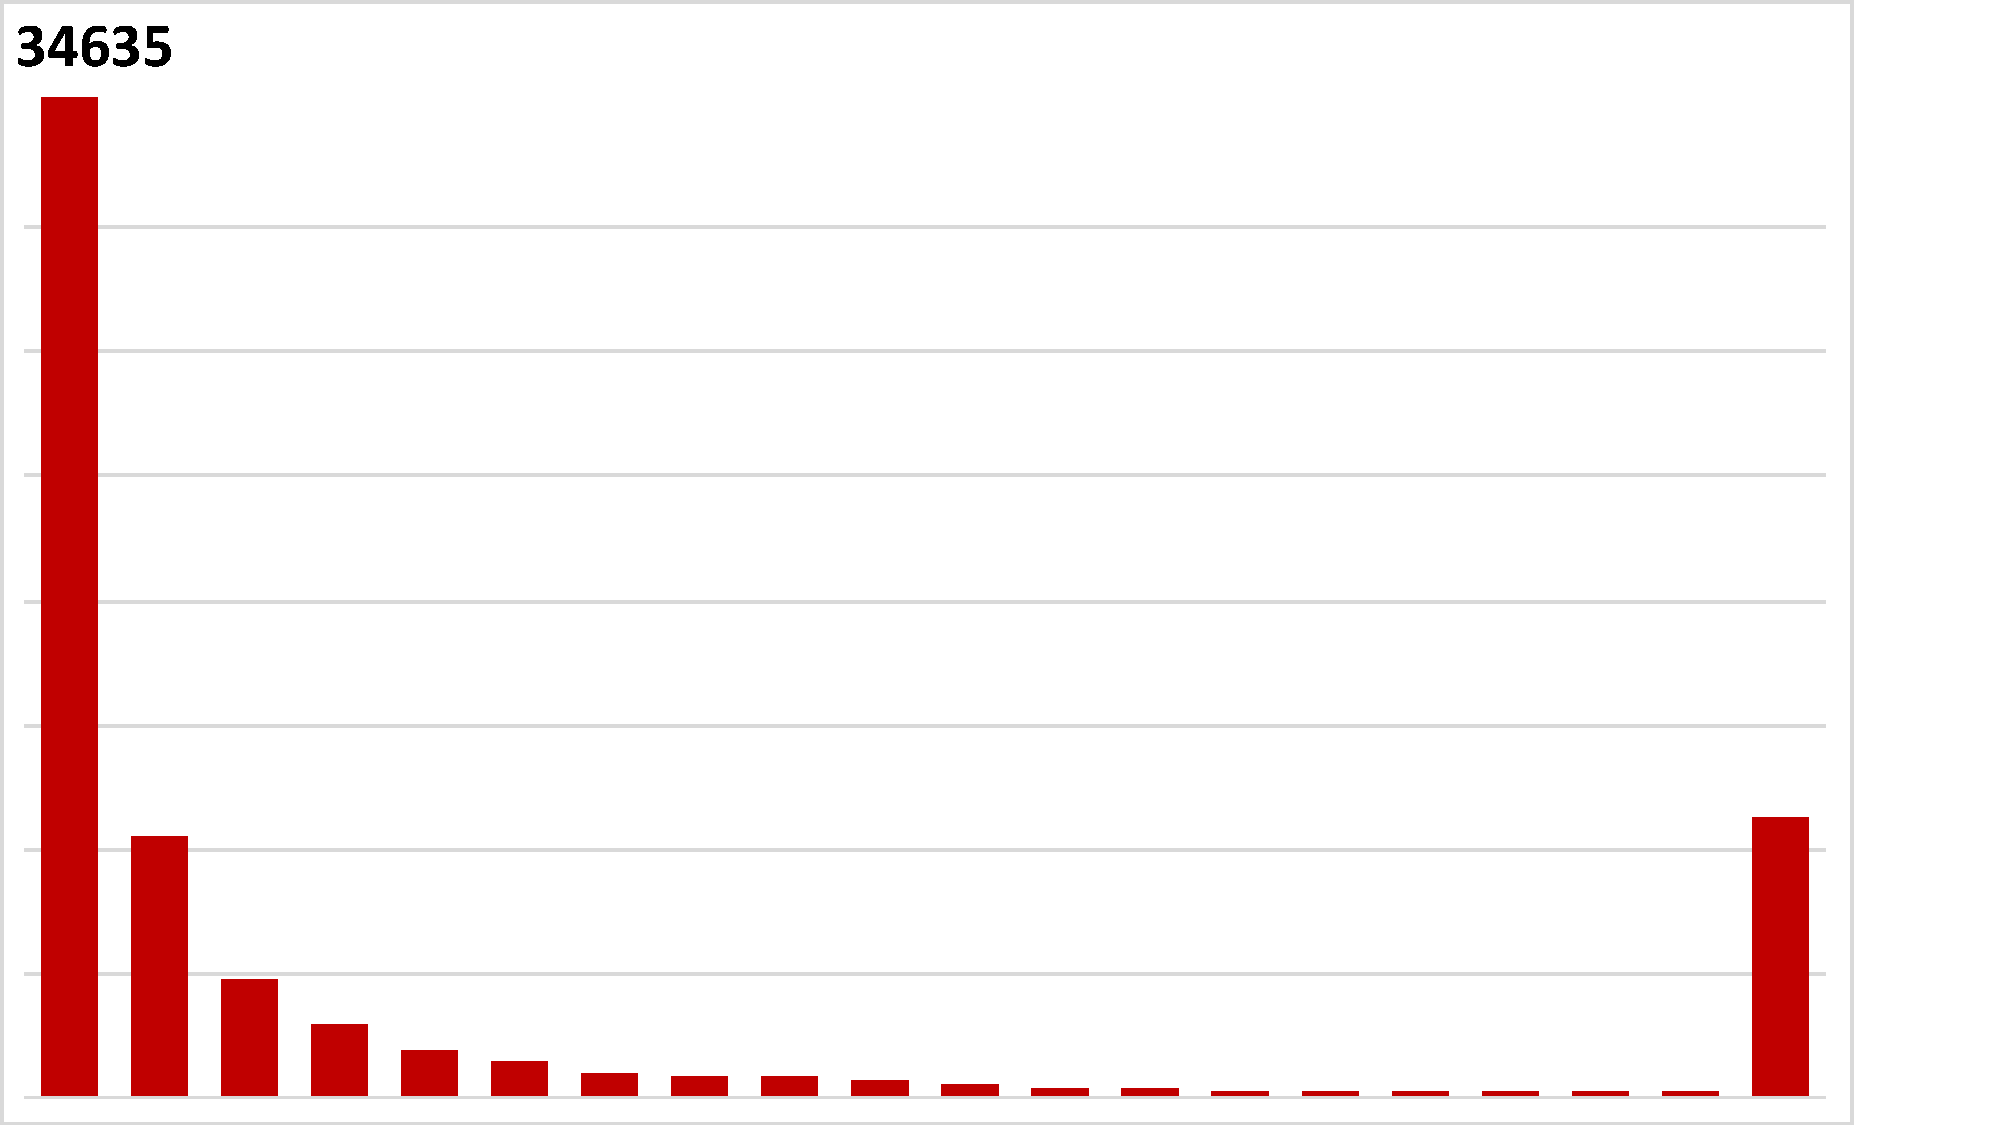
\includegraphics[width=0.95\linewidth, trim={0cm 0cm 2.5cm 0cm}, clip]{results/nyx/Lag200_1_Max.pdf}
\vspace{-2mm}
\captionof{subfigure}{Lag 200 Max$_{L2}$}
\end{minipage}
\end{framed}
\vspace{-2mm}
\captionof{figure}{\textbf{Nyx} experiment histograms for 50,000 test particle interpolation errors. Each plot has 20 bins, ranging from 0 to $>$0.44, with bar height encoding number of particles. Horizontal grid lines mark increments of 2,000.}
\label{fig:nyx_histograms}
\end{minipage}%
\vspace{-6mm}
\end{figure*}
